%!TEX root = ../report.tex
\documentclass[report.tex]{subfiles}
\begin{document}
    \chapter{Evaluation and Results}

    \section{Experiment Description}

    % Describe the experiments/evaluation you are performing to analyse your method.
    \paragraph*{Objective}

    % The primary objective of these experiments is to evaluate the efficacy of three multimodal sensor fusion deep neural network models on two diverse public datasets for object detection in a range of adverse weather conditions. This study aims to understand how tightly-coupled, data-driven multimodal sensor fusion can enhance object detection capabilities in environments where traditional methods may falter due to poor visibility and unpredictable weather elements.

    % This study aims to understand how tightly-coupled, data-driven multimodal sensor fusion can enhance object detection capabilities in environments where traditional methods may falter due to poor visibility and unpredictable weather elements.

    % This study aims to 
    % - Understand how tightly-coupled multimodal sensor fusion can enhance object detection capabilities in environments where conventional methods may falter due to poor visibility and unpredictable weather elements.
    % - Highlight the importance of complementary sensors suit for robust object detection in adverse weather conditions.

    % The primary objective of these experiments is to critically evaluate the efficacy of three multimodal sensor fusion deep neural network models on two diverse public datasets, specifically designed for object detection under a range of adverse weather conditions. This study is conducted with a dual aim. Firstly, it seeks to understand how tightly-coupled multimodal sensor fusion can significantly enhance object detection capabilities, particularly in environments where conventional methods may falter. This faltering is often due to poor visibility and the unpredictability of weather elements, which pose substantial challenges to standard detection techniques. Secondly, the study highlights the importance of employing a complementary suite of sensors. This approach is crucial for ensuring robust object detection in adverse weather conditions, suggesting that the integration of diverse sensor modalities can offer a more comprehensive and reliable solution in challenging environmental contexts.

    The primary objective of these experiments is to critically evaluate the efficacy of three multimodal sensor fusion deep neural network models on two diverse public datasets, specifically designed for object detection under a range of adverse weather conditions. Conducted with a dual aim, this study focuses on:

    \begin{itemize}
        \item \textbf{Understanding Tightly-Coupled Multimodal Sensor Fusion}: Investigating how the integration of multiple sensor types can significantly enhance object detection capabilities in environments where traditional methods are less effective. This is particularly relevant in scenarios with poor visibility and unpredictable weather elements, where standard detection techniques may struggle.
        \item \textbf{Highlighting the Importance of Complementary Sensors}: Emphasizing the necessity of employing a suite of complementary sensors for robust object detection in challenging weather conditions. This approach underlines the value of diverse sensor modalities working in concert to provide a more reliable and comprehensive solution for object detection in adverse environmental contexts.
    \end{itemize}

    \paragraph*{Relevance to Adverse Weather Conditions}

    This research tackles the significant challenges posed by adverse weather conditions such as heavy rain, fog, and snow, which greatly affect the accuracy of object detection systems essential in autonomous navigation and outdoor surveillance. Acknowledging the limitations of commonly used sensors like cameras and Lidar in inclement weather, contrasted with the robustness of radar, the study emphasizes integrating multimodal sensor data to bolster the robustness and reliability of object detection in these environments. This study provides a comprehensive overview and detailed analysis of existing top methods, elucidating their efficacy and limitations in diverse weather scenarios, thereby informing best practices in the field.

    \paragraph*{Experiment Overview}

    % TODO: if it is verbose, then shorten it
    \begin{itemize}
        \item \textbf{Objective of the Experiments:} The main aim of these experiments is to explore the strengths and weaknesses of using camera-only systems compared to systems that incorporate multiple sensor modalities, especially in challenging weather conditions.

        \item \textbf{Comparative Analysis of Fusion Architectures:} A key focus of the experiments is to compare the performance of tightly-coupled fusion architectures with conventional fusion architectures. This comparison is intended to provide insights into how different fusion methodologies impact the accuracy and reliability of object detection in adverse weather conditions.

        \item \textbf{Datasets Used for Evaluation:} The experiments utilize two major public datasets, namely nuScenes and DENSE, to provide a broad and comprehensive evaluation of the models. These datasets are particularly relevant as they include a variety of adverse weather conditions that pose challenges to object detection systems.

        \item \textbf{Performance Metrics and Evaluation:} The results of the experiments are quantified and presented using COCO style metrics. This choice of metric allows for a standardized comparison of model performance.

        \item \textbf{Weather-Specific Analysis:} Where possible, results are presented in the context of specific weather conditions. This approach helps to highlight how each model performs under various types of adverse weather, providing a more nuanced understanding of their capabilities and limitations.

        \item \textbf{Experiment Setup and Methodology:} Detailed descriptions of the experimental setup, including the specifics of the sensor arrays used, the configuration of the neural network models, and the criteria for evaluating their performance.

        \item \textbf{Interpretation of Results:} A thorough analysis of the experimental results, focusing on the efficacy of multimodal sensor fusion in improving object detection in adverse weather, and discussing the implications of these findings for the field of autonomous vehicles.
    \end{itemize}

    \section{Experimental Setup}

        \subsection{Hardware and Software Configuration}
        \begin{itemize}
            \item \textbf{Sensor Array Configuration:} The experiments utilized two multimodal datasets, which primarily comprise the following sensors:
                \begin{itemize}
                    \item RGB camera
                    \item LiDAR
                    \item Radar
                \end{itemize}
                These sensors were selected due to their varied capabilities in capturing environmental data under different weather conditions, as detailed in the respective dataset descriptions.

            \item \textbf{Computational Resources:} The experiments were conducted using HBRS University's High Performance Scientific Computing (HPC) \cite{hbrs_scientificComputing2023}, equipped multiple GPU devices, such as:
                \begin{itemize}
                    \item NVIDIA V100 GPU with 16GB memory
                    \item NVIDIA A100 GPU with 80GB memory
                \end{itemize}
                Additionally, for debugging purposes, lab computing resources featuring an NVIDIA RTX 3090 GPU with 24GB memory were utilized. For more details, please refer to the appendix \ref{appendix:gpu_details}. 

            \item \textbf{Software Environment:} The experiments employed the PyTorch framework for training and evaluation of the three methods. Specifically, two methods were implemented using the MMDetection framework, built on top of PyTorch, to facilitate the development of object detection models. Below Table \ref{tab:pytorch_versions} shows the PyTorch versions used for each method.
            
            \begin{table}[h]
                \centering
                \caption{PyTorch and CUDA versions}
                \begin{tabular}{|l|l|l|}
                \hline
                \textbf{Methods} & \textbf{PyTorch} & \textbf{CUDA} \\ \hline
                SAF-FCOS & 1.12 & 11.6 \\ \hline
                HRFuser & 1.10 & 10.2 / 11.1 \\ \hline
                MT-DETR & 1.10 & 11.1 \\ \hline
                \end{tabular}
                \label{tab:pytorch_versions}
            \end{table}
        \end{itemize}

        \subsection{Datasets}
        \begin{itemize}
            \item \textbf{Dataset Description:} A detailed description of the datasets used in the experiments is provided in Section~\ref{sec:available_datasets}. It is important to note that, although both datasets offer 360-degree perception coverage, the methods employed in this study utilized only the front-view sensors for training.

            \item \textbf{Data Preprocessing:} In addition to the projection methods outlined in Section~\ref{sec:selected_methods}, the experiments incorporated basic data augmentation techniques: RandomFlip, RandomCrop, and RandomDrop. Note that `RandomDrop' is an augmentation method where sensor streams in multimodal architectures are randomly omitted with a specified probability. The table below outlines the specific augmentation techniques employed for each method in the experiments:
                \begin{table}[h]
                    \centering
                    \caption{Methods and augmentation techniques}
                    \begin{tabular}{|l|l|}
                    \hline
                    \textbf{Methods} & \textbf{Augmentation Techniques} \\ \hline
                    SAF-FCOS & RandomFlip, Crop, Resize \\ \hline
                    HRFuser & RandomFlip, Crop, Resize, RandomDrop \\ \hline
                    MT-DETR & RandomFlip, RandomCrop, Resize \\ \hline
                    \end{tabular}
                    \label{tab:methods_augmentation}
                \end{table}

            \item \textbf{Dataset Split:} 
            
            \paragraph*{SAF-FCOS}

            The method limits its focus on detecting vehicular obstacles such as — bicycles, cars, motorcycles, buses, trailer, and trucks—collectively categorized as 'vehicles' for simplified classification. Pedestrians are excluded due to radar detection limitations in the nuScenes dataset. Emphasis is placed on front camera data from nuScenes, with the dataset split detailed in Figure \ref{fig:saffcos_data_split}.

            \begin{figure}[h!]
                \centering
                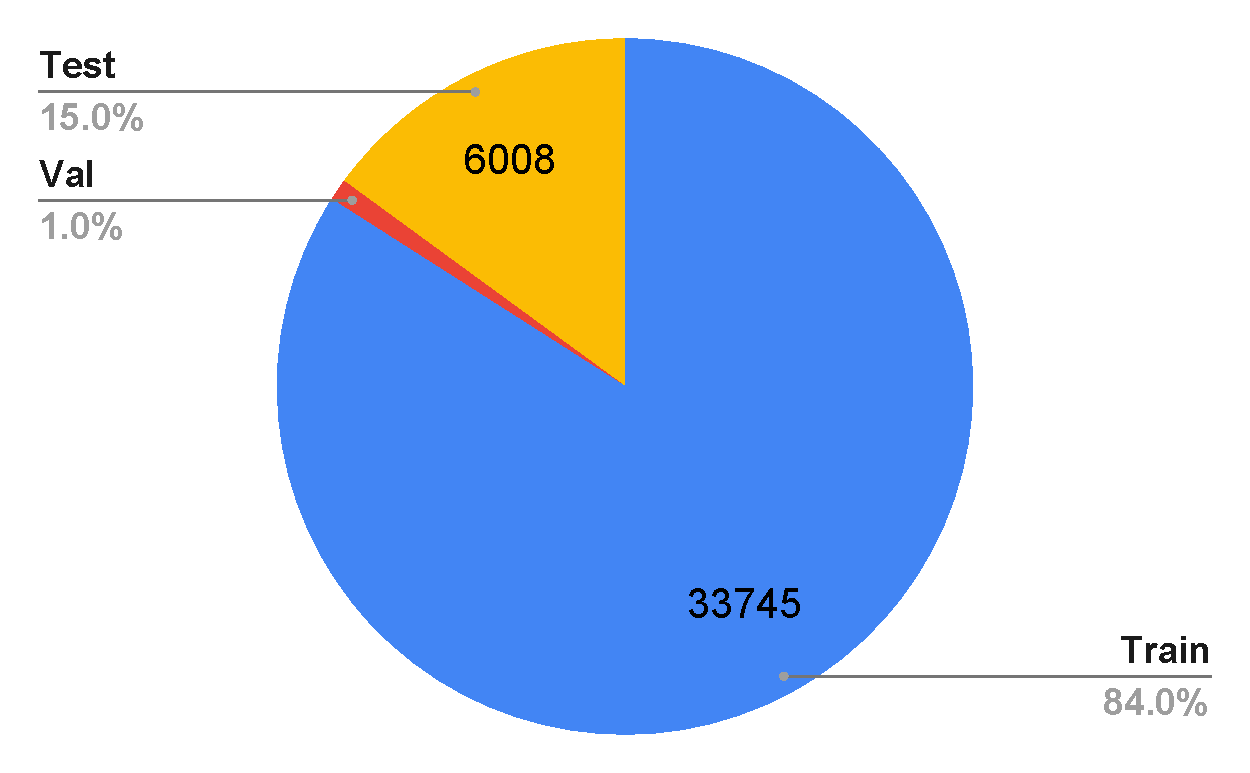
\includegraphics[width=0.6\textwidth]{images/methods/saf_fcos/data_split.pdf}
                \caption{Data split of nuScenes dataset. Total samples: 40157. Note: this is a custom dataset split chosen by the authors.}
                \label{fig:saffcos_data_split}
            \end{figure}

            \paragraph*{HRFuser}

            The original HRFuser approach employs ten superclasses derived from the nuScenes dataset for its training and evaluation protocols. Table \ref{tab:hrfuser_classes_nuscenes} delineates the correspondence between nuScenes and HRFuser class categorizations. To facilitate a direct comparison with SAF-FCOS, we adopted identical class designations and data partitions as delineated in SAF-FCOS. This alignment extends to the annotation process. As detailed in Section \ref{subsec:nuscenes_dataset}, the nuScenes dataset omits 2D annotations for its test set. Consequently, the SAF-FCOS framework generated proprietary annotations for this subset by leveraging an augmented version of FCOS supplemented with manual adjustments. To synchronize our performance metrics, we have created a custom annotation conversion script that reformats SAF-FCOS annotations into the HRFuser schema. This utility underscores the variance in annotation formats within multimodal datasets, despite both methodologies utilizing COCO-style annotations. The conversion script is accessible in our code repository for replication and further research endeavors.

            \begin{table}[h]
                \centering
                \caption{Mapping from nuScenes classes to HRFuser classes \cite{caesar2020nuscenes}}
                \begin{tabular}{|l|l|}
                \hline
                \textbf{NuScenes Class} & \textbf{Mapped Class} \\ \hline
                vehicle.car & car \\ \hline
                vehicle.truck & truck \\ \hline
                vehicle.trailer & trailer \\ \hline
                vehicle.bus.bendy & bus \\ \hline
                vehicle.bus.rigid & bus \\ \hline
                vehicle.construction & construction\_vehicle \\ \hline
                vehicle.bicycle & bicycle \\ \hline
                vehicle.motorcycle & motorcycle \\ \hline
                human.pedestrian.child & pedestrian \\ \hline
                human.pedestrian.adult & pedestrian \\ \hline
                human.pedestrian.construction\_worker & pedestrian \\ \hline
                human.pedestrian.police\_officer & pedestrian \\ \hline
                movable\_object.trafficcone & traffic\_cone \\ \hline
                movable\_object.barrier & barrier \\ \hline
                \end{tabular}
                \label{tab:hrfuser_classes_nuscenes}
            \end{table}
                

            For DENSE dataset, the method uses 3 classes for training and evaluation, namely Car, Pedestrian, and Cyclist, Table \ref{tab:hrfuser_classes_dense} shows the mapping from DENSE classes to HRFuser classes. The dataset split is shown in Figure \ref{fig:hrfuser_data_split_dense}.

            \begin{table}[h]
                \centering
                \caption{Mapping from DENSE classes to HRFuser classes \cite{broedermann2022hrfuser}}
                \begin{tabular}{|l|l|}
                \hline
                \textbf{DENSE Class} & \textbf{Mapped Class} \\ \hline
                PassengerCar         & Car                   \\ \hline
                Pedestrian           & Pedestrian            \\ \hline
                RidableVehicle       & Cyclist               \\ \hline
                Large Vehicle        & Car                   \\ \hline
                DontCare             & DontCare              \\ \hline
                \end{tabular}
                
                \label{tab:hrfuser_classes_dense}
            \end{table}

            \begin{figure}[h!]
                \centering
                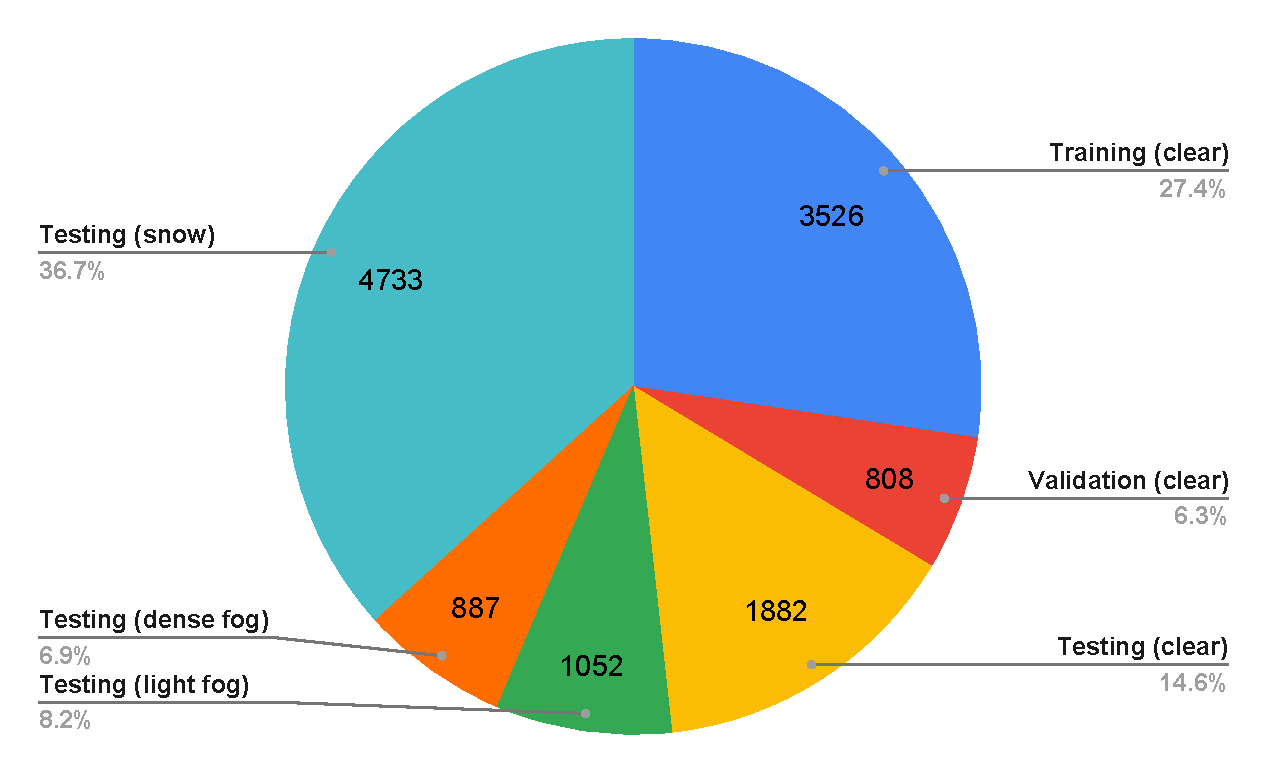
\includegraphics[width=0.7\textwidth]{images/datasets/dense/dataset_split.pdf}
                \caption{Data split for DENSE dataset. Total samples: 12888. Note: all methods use clear weather data for training and validation, and use adverse weather data for testing.}
                \label{fig:hrfuser_data_split_dense}
            \end{figure}

            \paragraph*{MT-DETR}

            The MT-DETR model adopts a distinct class categorization for training and evaluation purposes, on the DENSE dataset. Specifically, it combines the 'Car' and 'Cyclist' classes into a unified 'Vehicle' category while maintaining 'Pedestrian' as a standalone class. Consequently, the MT-DETR conducts its training and evaluation processes on these two distinct classes. It is important to note that MT-DETR follows the same dataset partitioning as utilized in the HRFuser framework, which is delineated in Figure \ref{fig:hrfuser_data_split_dense}.

                
        \end{itemize}

        \subsection{Model Configuration and Training}
        \begin{itemize}
            
            \item \textbf{Training Parameters:} The Table \ref{tab:experiment_training_parameters} below represents typical training configurations for each method employed in this project. However, the original settings varied from these due to GPU computational constraints. In addition, all methods implement learning rate decay and warmup schemes. It should be noted that the asterisk (*) in the table denotes the total batch size when the model is trained across multiple GPUs.
            
            The model checkpoint with the lowest validation loss is used for evaluation on the test set. The training parameters for each method are detailed below:

            \begin{table}[h]
                \centering
                \caption{Training parameters. (*) denotes total batch size for models trained on multiple GPUs.}
                \begin{tabular}{|l|l|l|l|l|l|}
                \hline
                \textbf{Methods} & \textbf{Optimizer} & \textbf{Learn. Rate} & \textbf{Batch Size} & \textbf{Epochs} & \textbf{Input (WxH)} \\ \hline
                SAF-FCOS         & SGD                & 0.001                & 8                   & 12              & 1333 x 800           \\ \hline
                HRFuser (nuScenes) & AdamW             & 0.0003               & 12*                 & 12              & 640x384              \\ \hline
                HRFuser (DENSE)    & AdamW             & 0.001                & 12*                 & 60              & 1284x384             \\ \hline
                MT-DETR            & AdamW             & 0.0001               & 1                   & 36              & 1333 x 800           \\ \hline
                \end{tabular}
                \label{tab:experiment_training_parameters}
            \end{table}
            
            
            \item \textbf{Evaluation Metrics:} For the evaluation of the models, the COCO style evaluation metrics were adopted. For each method and its respective configuration, we provide comprehensive details including the total number of model parameters, floating point operations, and the inference time. The details are described in Section~\ref{sec:metrics}.
            
            For every method and in all experimental combinations, the model inference confidence threshold is set to 0.3, in accordance with the threshold specified in the original paper.
        \end{itemize}

        

        
        \subsection{Experimental Procedure}
        \begin{itemize}
            \item \textbf{Testing Protocol:} To facilitate a comprehensive quantitative analysis, all models were evaluated using test sets from both datasets. For comparative purposes, Average Precision (AP) and Average Recall (AR) metrics were employed. Additionally, the models were assessed in terms of complexity, considering aspects such as the number of model parameters, floating-point operations, and inference time. For qualitative analysis, images showcasing model predictions alongside ground truth on the test sets were provided for each comparison.
            \item \textbf{All Experiments Combinations:} The table referenced as Table \ref{tab:experiment_combinations} presents all the combinations of experiments conducted for each method. In it, each tick mark indicates the combinations available for each respective method. 

            \begin{table}[h!]
                \centering
                \caption{Overview of experiment combinations. 'Extra' indicates additional modalities used.}
                \begin{tabular}{|l|c|c|c|c|c|c|c|}
                \hline
                \textbf{Methods} & \textbf{Early} & \textbf{Middle} & \textbf{Tightly-coupled} & \textbf{Camera} & \textbf{Radar} & \textbf{Lidar} & \textbf{Extra} \\ \hline
                SAF-FCOS & $\times$ & $\checkmark$ & $\times$ & $\checkmark$ & $\checkmark$ & $\times$ & $\times$ \\ \hline
                HRFuser & $\times$ & $\times$ & $\checkmark$ & $\checkmark$ & $\checkmark$ & $\checkmark$ & Gated \\ \hline
                MT-DETR & $\checkmark$ & $\checkmark$ & $\checkmark$ & $\checkmark$ & $\checkmark$ & $\checkmark$ & Time \\ \hline
                \end{tabular}
                \label{tab:experiment_combinations}
                \end{table}

            
            \textbf{NOTE: The majority of the experiments were carried out utilizing the DENSE dataset in conjunction with the MT-DETR method. Due to computational complexities and resource constraints, it is not feasible to evaluate every possible combination.}
                
        \end{itemize}
        
    \section{Results}

    \subsection{SAF-FCOS vs. HRFuser}

    In this section, we conduct an evaluation of the performance of two distinct methods on the nuScenes test dataset. The first method, SAF-FCOS, utilizes a Middle Fusion architecture, while the second method, HRFuser, is built upon a Tightly-Coupled Fusion architecture. It is important to note that this Experiment is focused only on the fusion of Camera and Radar sensor data. The results are presented in accordance with COCO-style metrics, as outlined in Table \ref{tab:coco_metrics}.

    \begin{figure}[h!]
        \centering
        \begin{subfigure}[b]{0.45\textwidth}
            \centering
            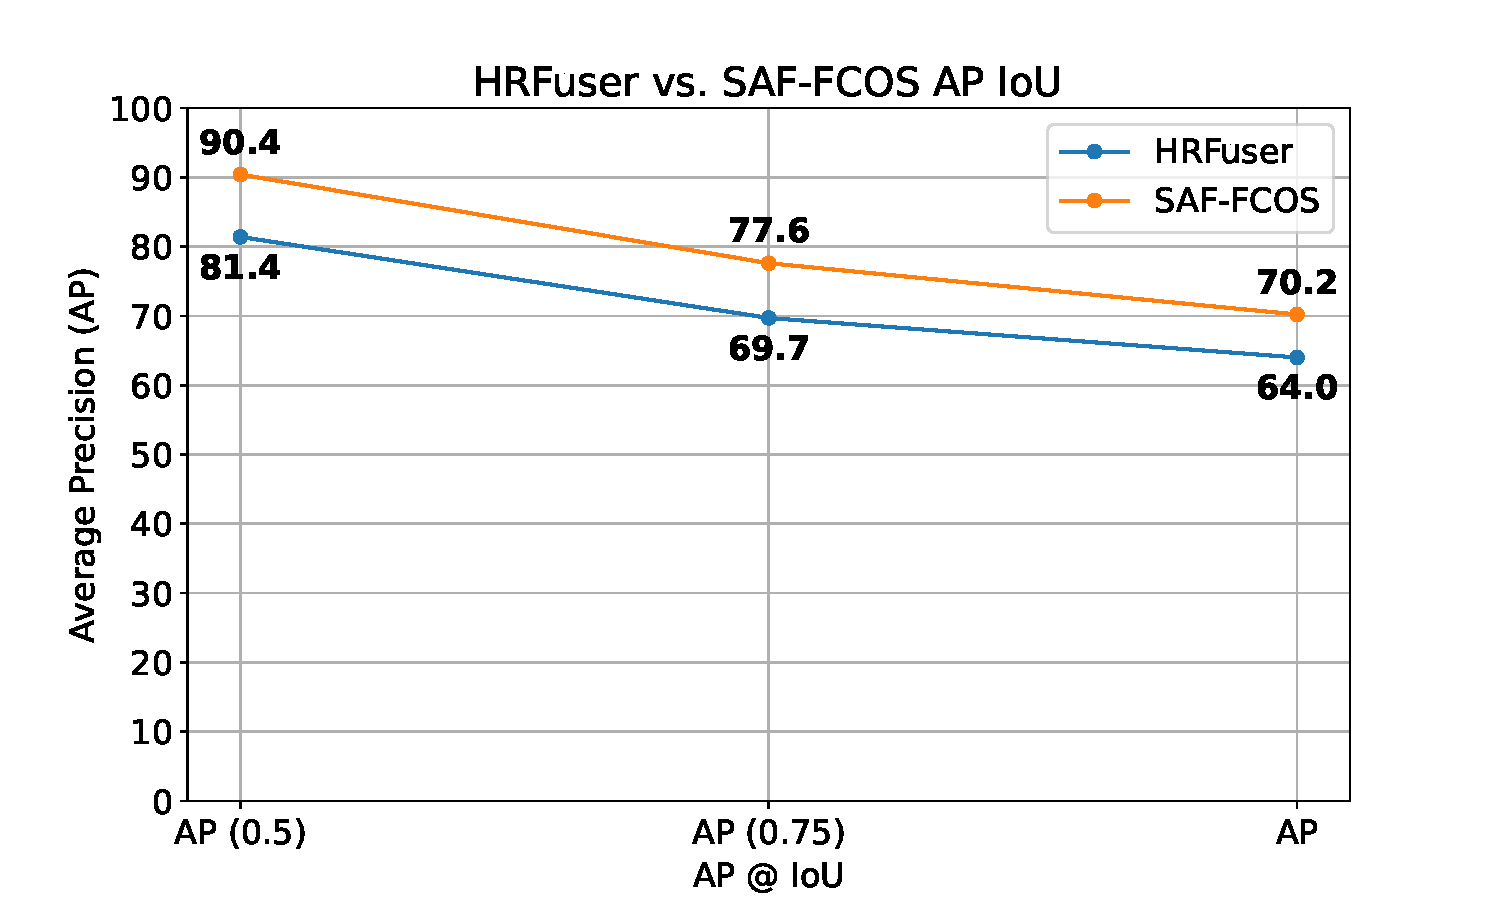
\includegraphics[width=\textwidth]{images/results/saf_vs_hrfuser/ap_iou.pdf}
            \caption{Average Precision (AP)}
            \label{fig:saf_vs_hrfuser_ap_iou}
        \end{subfigure}
        \hfill % adds horizontal space between figures
        \begin{subfigure}[b]{0.45\textwidth}
            \centering
            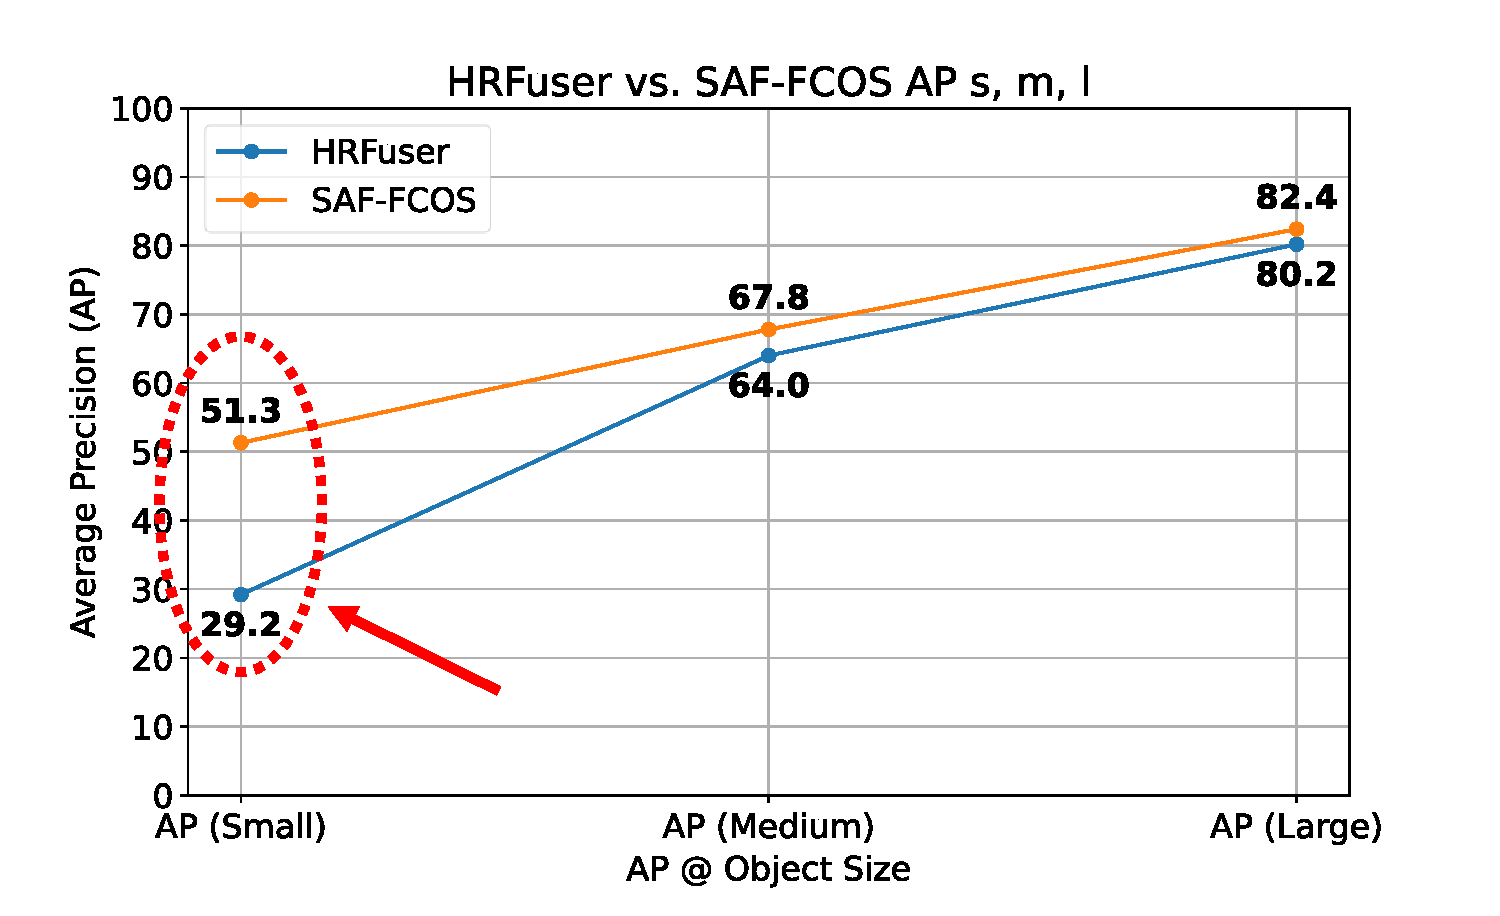
\includegraphics[width=\textwidth]{images/results/saf_vs_hrfuser/ap_sml_anno.pdf}
            \caption{Average Precision (AP) at S, M, L}
            \label{fig:saf_vs_hrfuser_ap_sml}
        \end{subfigure}
        \vspace{1em} % adds vertical space between rows
        \begin{subfigure}[b]{0.45\textwidth}
            \centering
            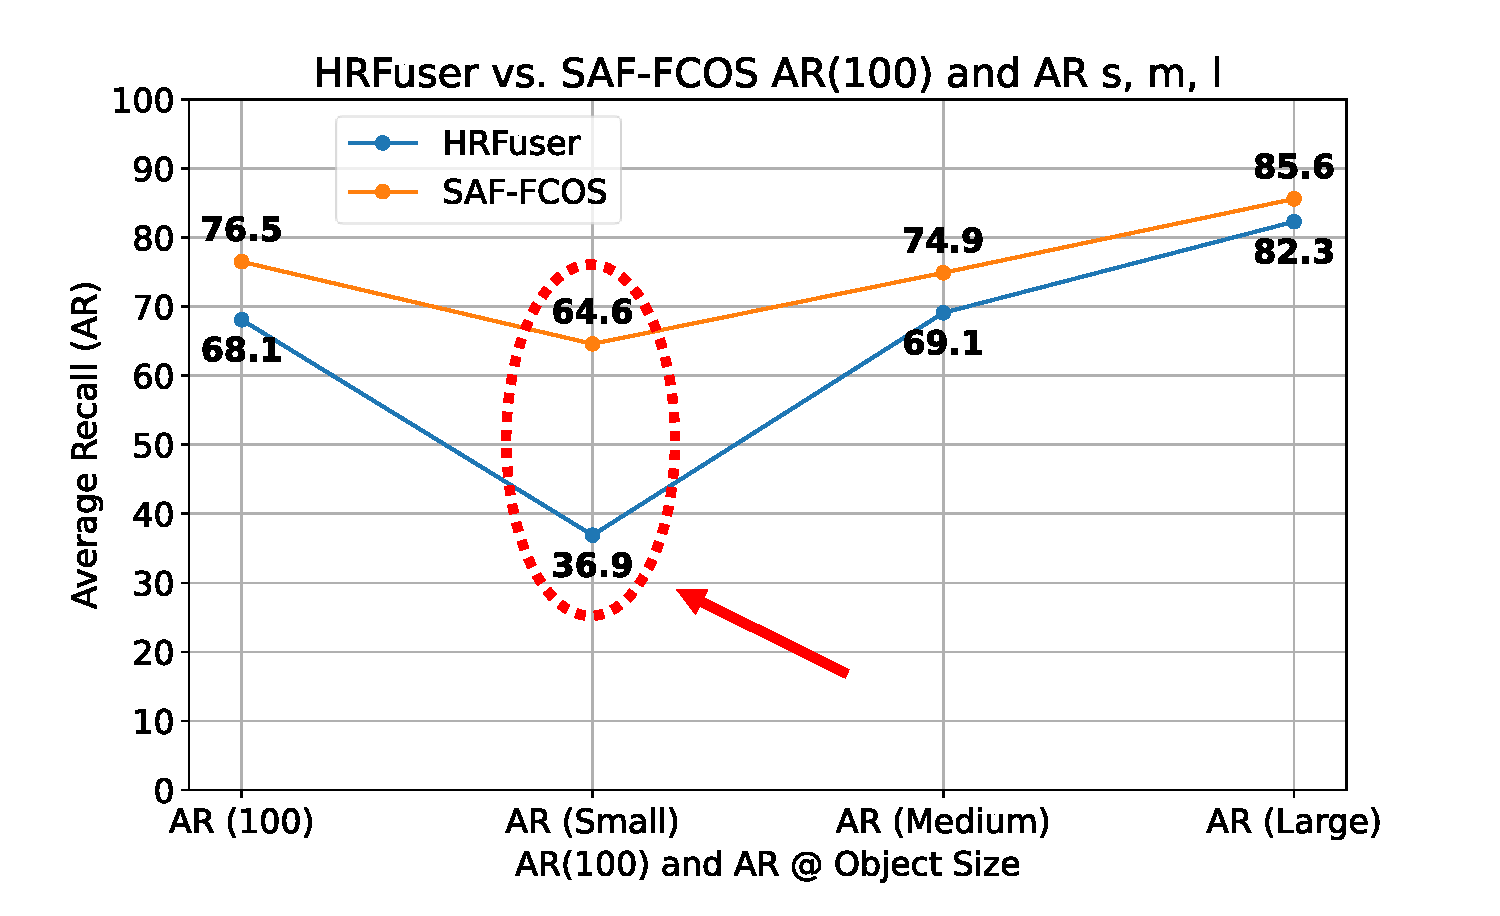
\includegraphics[width=\textwidth]{images/results/saf_vs_hrfuser/ar_anno.pdf}
            \caption{Average Recall (AR)}
            \label{fig:saf_vs_hrfuser_ar}
        \end{subfigure}
        \hfill
        \begin{subfigure}[b]{0.45\textwidth}
            \centering
            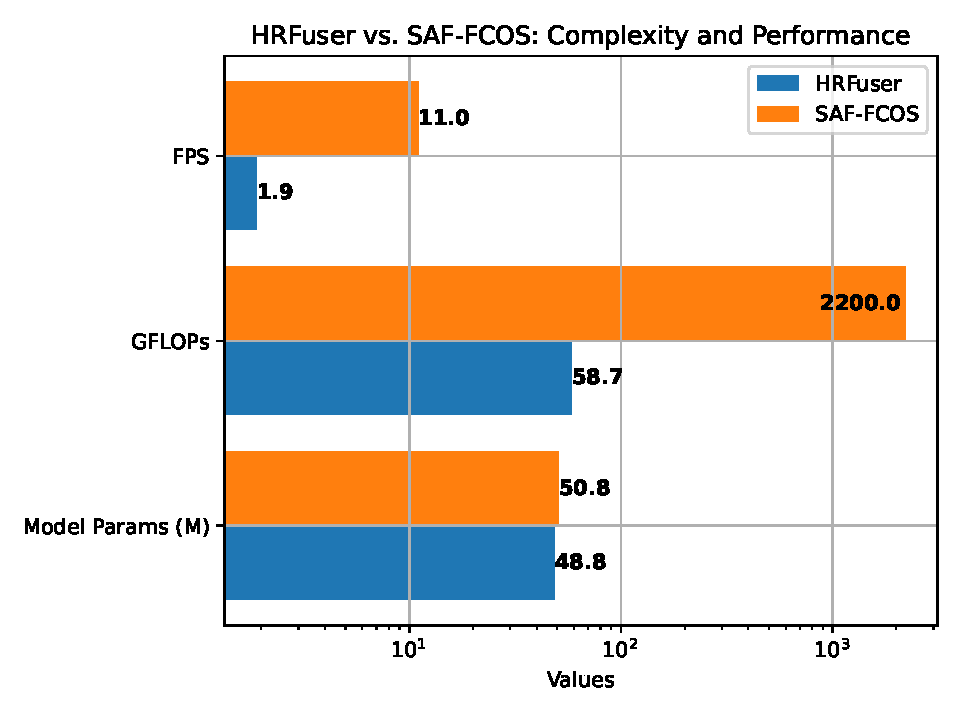
\includegraphics[width=\textwidth]{images/results/saf_vs_hrfuser/model_complexity.pdf}
            \caption{Model Complexity}
            \label{fig:saf_vs_hrfuser_model_complexity}
        \end{subfigure}
        \caption{Comparative Analysis: (a) Comparison on Average Precision (AP) at different IoU thresholds. Note AP@0.5:0.05:0.95 is the mean AP across all IoU thresholds. (b) Comparison on Average Precision (AP) at different object sizes. (c) Comparison on Average Recall (AR) with AR(100) and at different object sizes. (d) Comparison in terms of model parameters (M), computational complexity (GFLOPs), and frame rate (FPS).}
        \label{fig:comparative_analysis}
    \end{figure}

    % From the quantitative comparison, it can be clearly concluded that SAF-FCOS outperforms HRFuser in all metrics. It is important to note here that despite having slightly more model parameters (+2 M) than HRFuser, the FPS value is significantly higher, 11 vs. 1.9 FPS. The possible reason could be due to the fact that SAF-FCOS uses single-stage detector while HRFuser uses two-stage detector. However, surprisingly, from the model complexity Fig. \ref{fig:saf_vs_hrfuser_model_complexity} (d), it seems that SAF-FCOS having a huge x36 times more floating-point operations than its counterpart HRFuser. One possible reason behind this is that floating-point operations are highly dependent on the input size of the sample. In this comparison, as described in the Table \ref{tab:experiment_training_parameters}, SAF-FCOS is using much larger input than the HRFuser. So for this reason, the GFLOPs value is much higher than HRFuser. Also from the annotated figures \ref{fig:comparative_analysis} (b) and (c), it is observable that the performance gap between SAF-FCOS and HRFuser is much larger for small objects. This points to the advantage of using Spatial Attention Fusion (SAF) block in the SAF-FCOS architecture, which was specifically added to gain as much as information possible from the sparse radar data. So overall, for this particular experiment, it seems that Middle Fusion architecture is more robust than Tightly-Coupled Fusion architecture on nuScenes test dataset.


    The comparative analysis demonstrates a clear superiority of SAF-FCOS over HRFuser across all metrics. Notably, SAF-FCOS exhibits a remarkable frame rate of 11 FPS, significantly outstripping HRFuser's 1.9 FPS, despite having a marginally higher model parameter count (+2M). This performance disparity is likely attributable to SAF-FCOS's utilization of a single-stage detector, as opposed to HRFuser's two-stage approach. Contrasting this, an examination of model complexity, as illustrated in Fig. \ref{fig:saf_vs_hrfuser_model_complexity} (d), reveals an unexpected finding: SAF-FCOS requires substantially more floating-point operations — a factor of 36 times greater than HRFuser. A plausible explanation for this discrepancy is the dependency of floating-point operations on input size. As indicated in Table \ref{tab:experiment_training_parameters}, SAF-FCOS processes considerably larger inputs compared to HRFuser, resulting in a heightened GFLOPs value.

    Further scrutiny, particularly of the annotated figures \ref{fig:comparative_analysis} (b) and (c), discloses a more pronounced performance differential in the detection of smaller objects. This observation underscores the efficacy of the Spatial Attention Fusion (SAF) block integrated within the SAF-FCOS framework. The SAF block's inclusion is a strategic enhancement aimed at maximizing the extraction of information from sparse radar data. Consequently, in this specific experimental context using the nuScenes test dataset, the Middle Fusion architecture, exemplified by SAF-FCOS, demonstrates a robustness surpassing that of the Tightly-Coupled Fusion architecture, as represented by HRFuser.

    \paragraph*{Qualitative Analysis}

    The effectiveness of SAF-FCOS and HRFuser methods in different weather conditions is clearly demonstrated in the nuScenes test set. Figure \ref{fig:saf_vs_hrfuser} shows various scenarios. The first row shows how these methods detect objects in bright daylight, where many objects are present. The second row focuses on night conditions, where it's harder to see objects due to low light. The third row shows detection during rain, with the camera lens affected by water, yet both models still successfully identify objects. Importantly, rows four and five compare the detection of small, distant objects. Here, SAF-FCOS proves to be more effective than HRFuser, highlighting its better performance in spotting smaller objects that are far away. This performance underscores the significance of the long detection range of radar sensors, with SAF-FCOS effectively extracting relevant information from these challenging scenarios. This comparison is crucial for understanding how each method performs under different conditions.

    \begin{figure}[h!]
        \centering
        % Row 1
        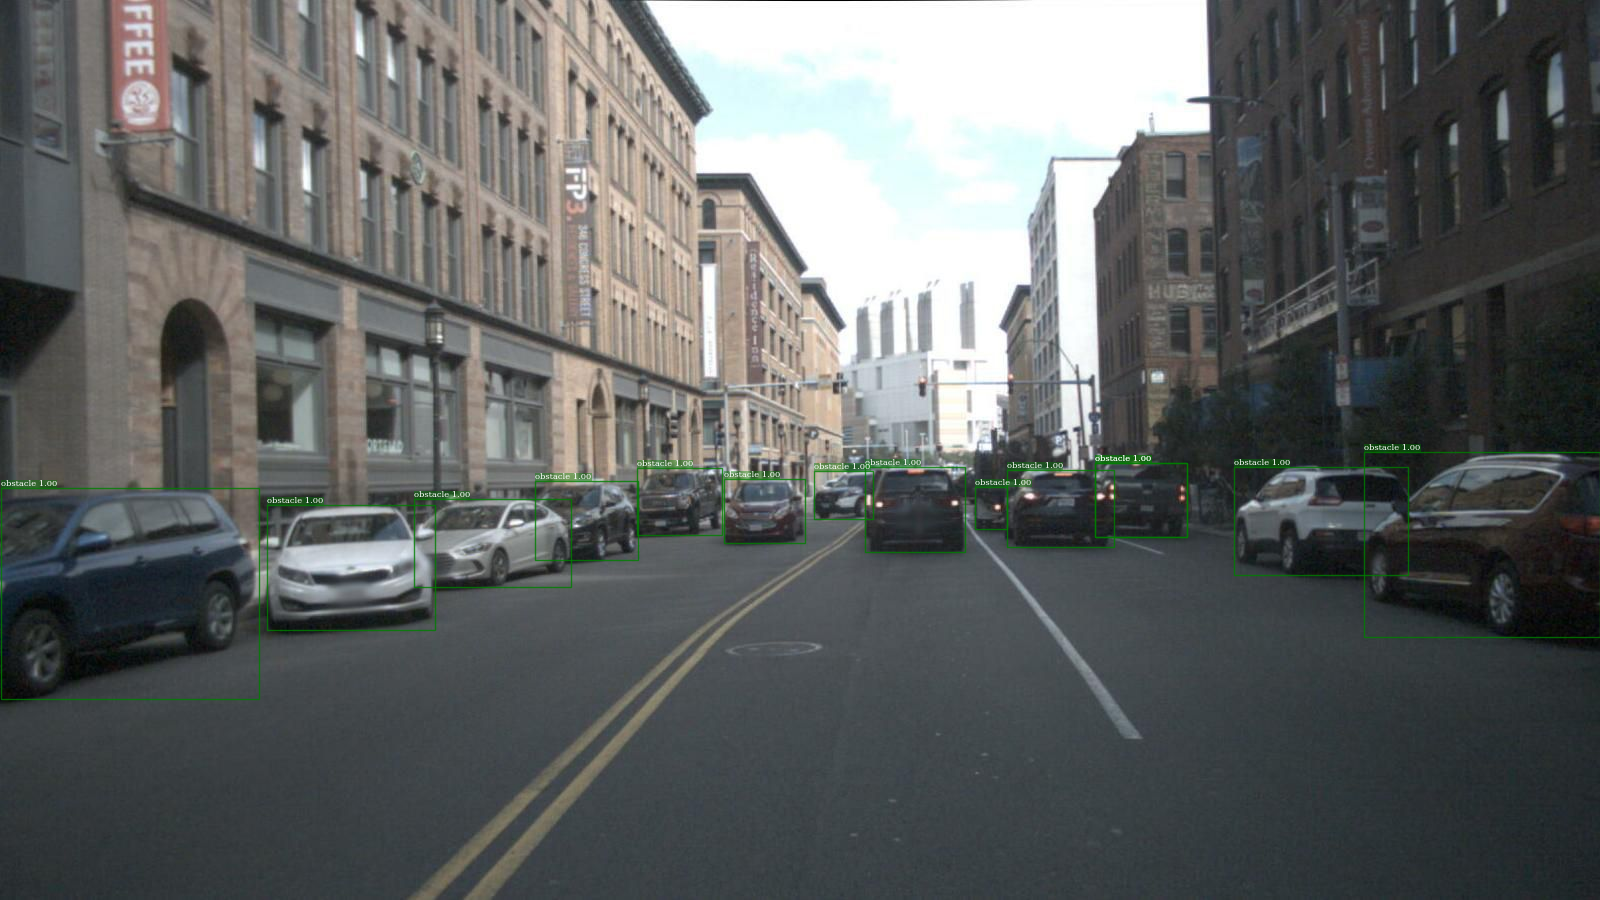
\includegraphics[width=0.3\textwidth]{images/results/saf_vs_hrfuser/samples/s3_day_regular/n008-2018-08-01-15-34-25-0400__CAM_FRONT__1533152655412404_gt.png}\hfill
        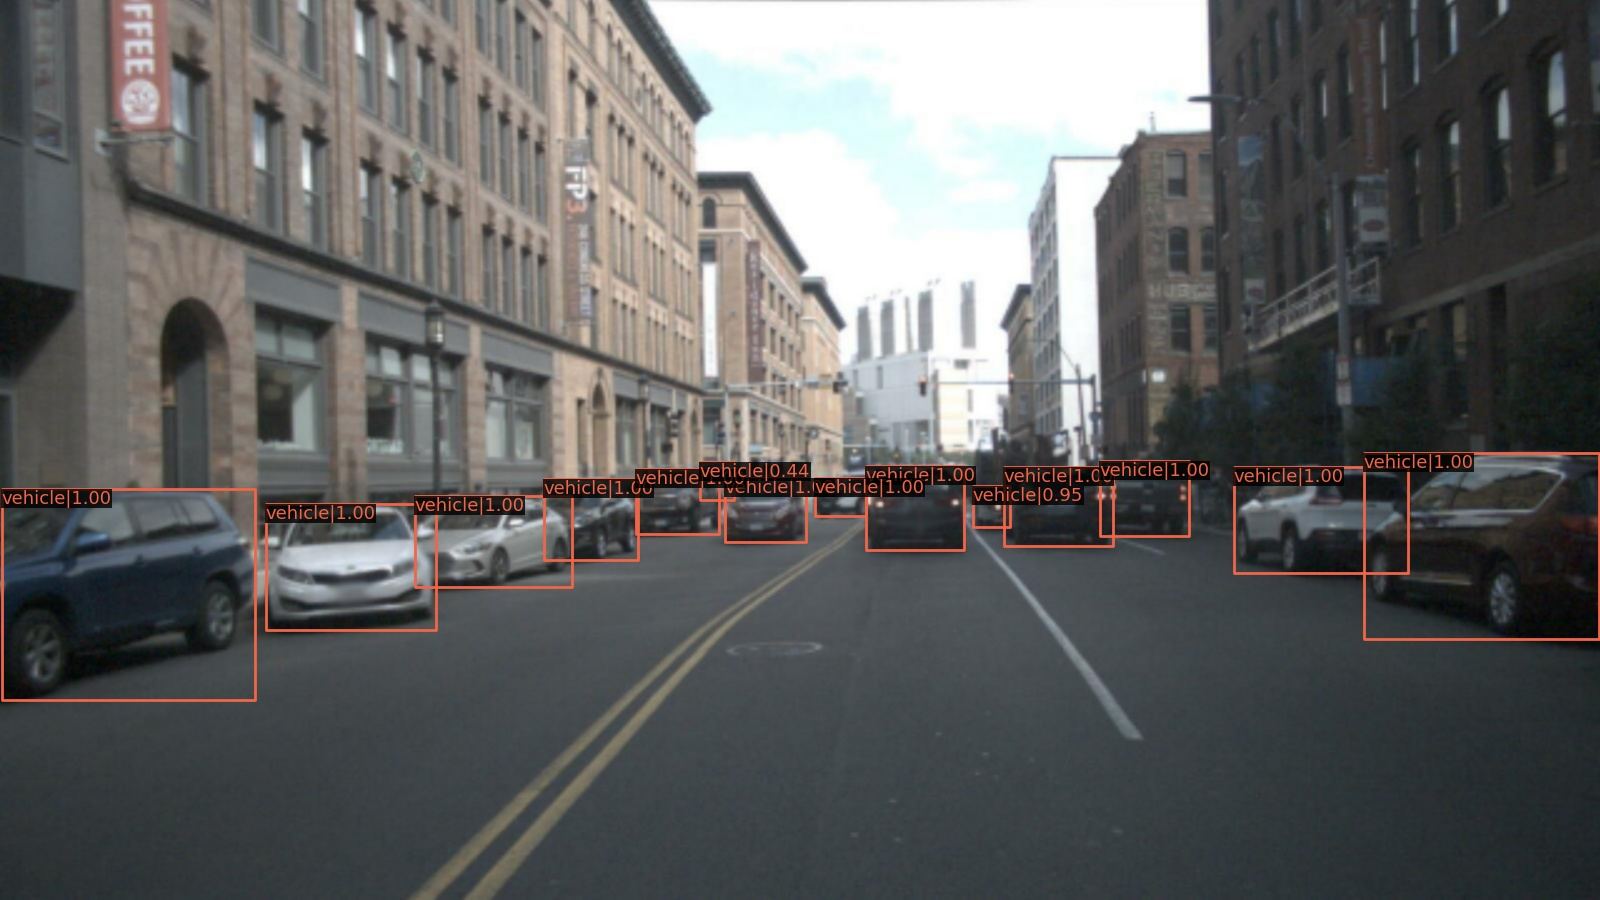
\includegraphics[width=0.3\textwidth]{images/results/saf_vs_hrfuser/samples/s3_day_regular/n008-2018-08-01-15-34-25-0400__CAM_FRONT__1533152655412404_former.jpg}\hfill
        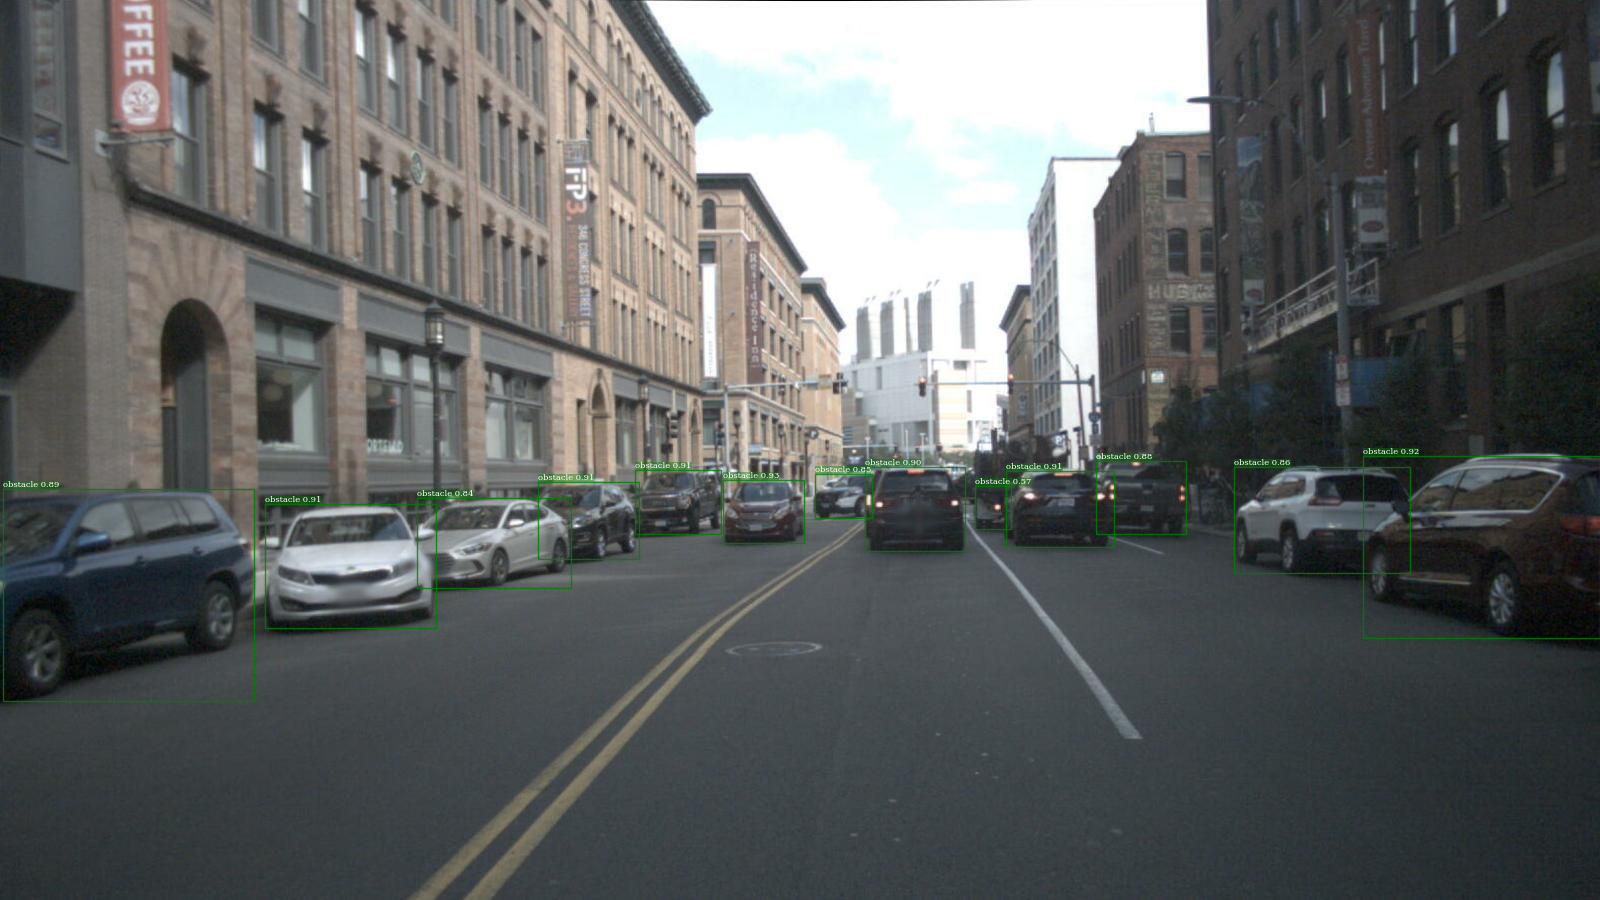
\includegraphics[width=0.3\textwidth]{images/results/saf_vs_hrfuser/samples/s3_day_regular/n008-2018-08-01-15-34-25-0400__CAM_FRONT__1533152655412404.png}
      
        % Row 2
        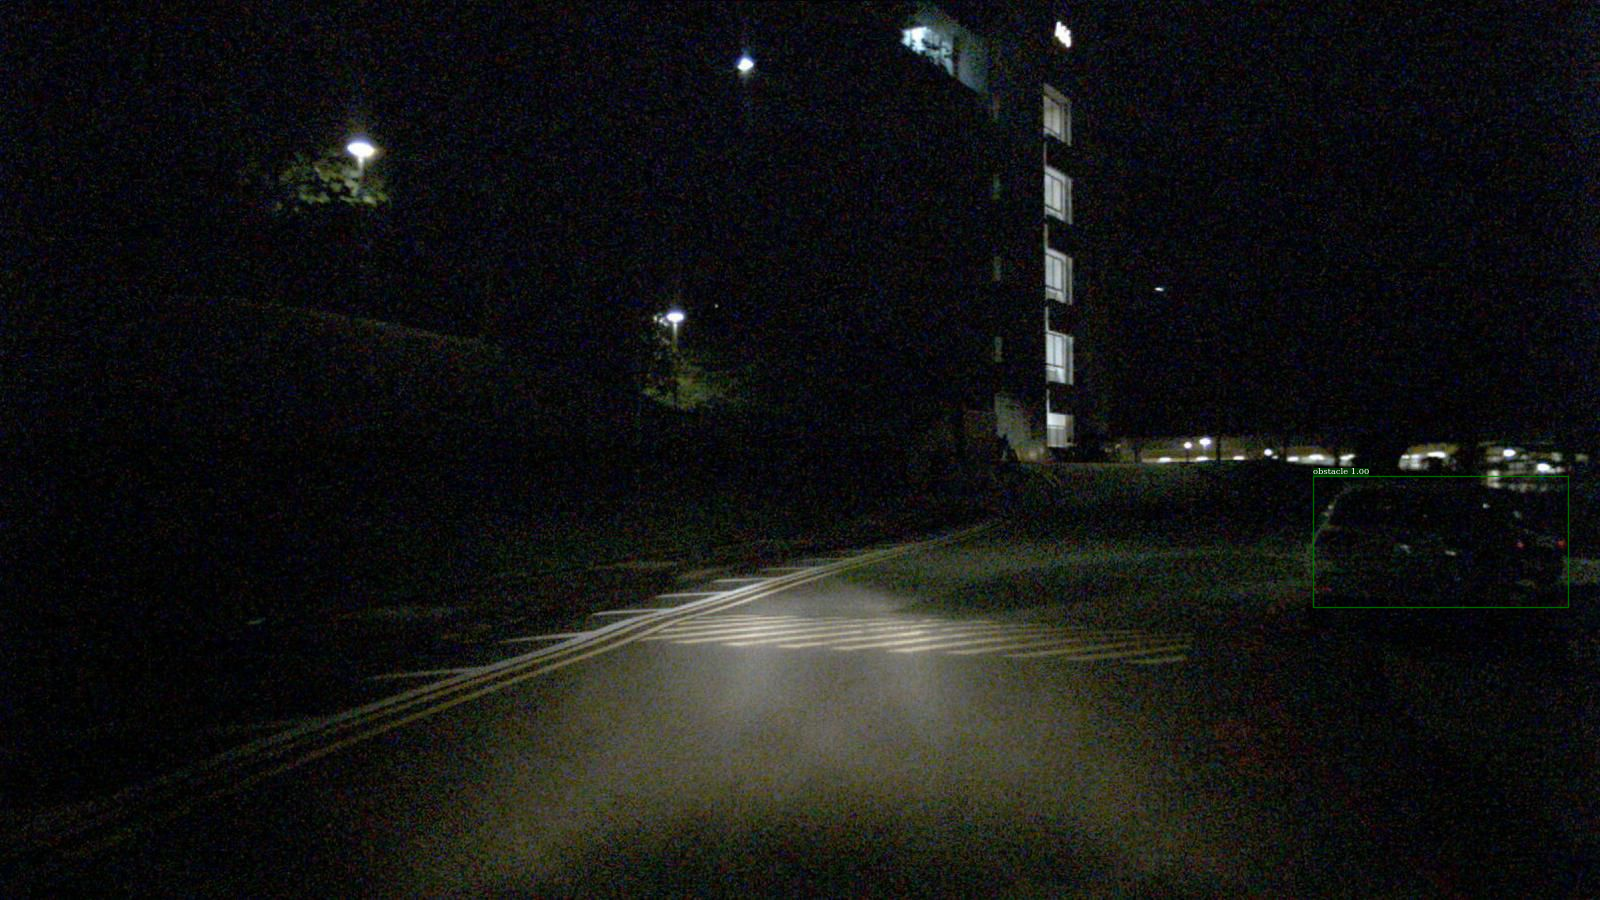
\includegraphics[width=0.3\textwidth]{images/results/saf_vs_hrfuser/samples/s4_night_reg/n015-2018-11-14-19-52-02+0800__CAM_FRONT__1542196675862460_gt.png}\hfill
        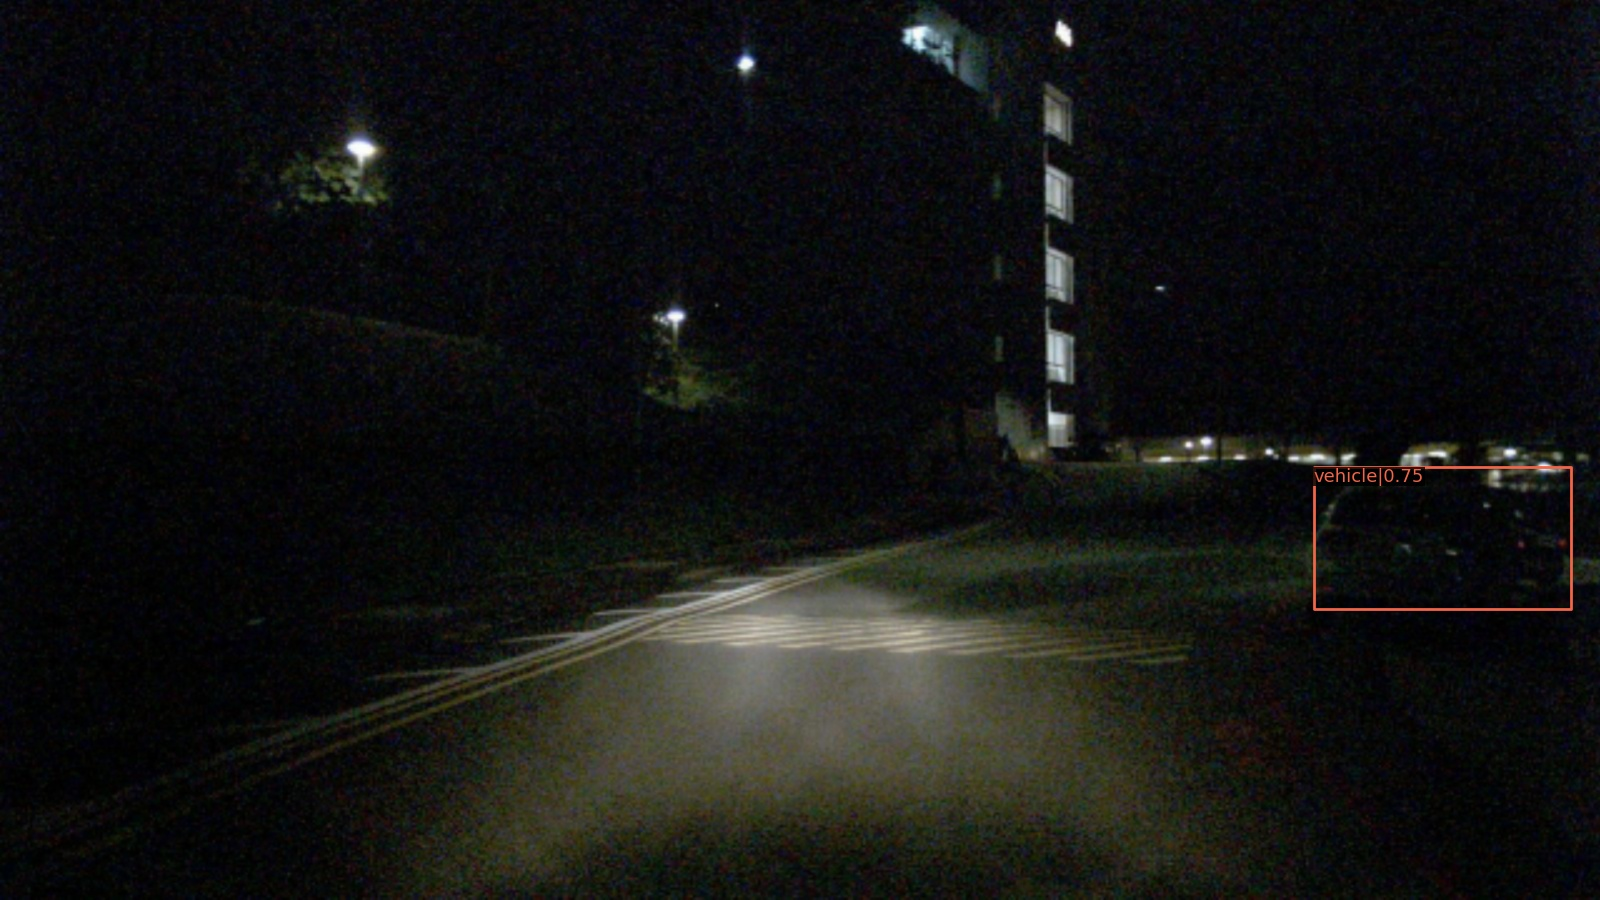
\includegraphics[width=0.3\textwidth]{images/results/saf_vs_hrfuser/samples/s4_night_reg/n015-2018-11-14-19-52-02+0800__CAM_FRONT__1542196675862460_former.jpg}\hfill
        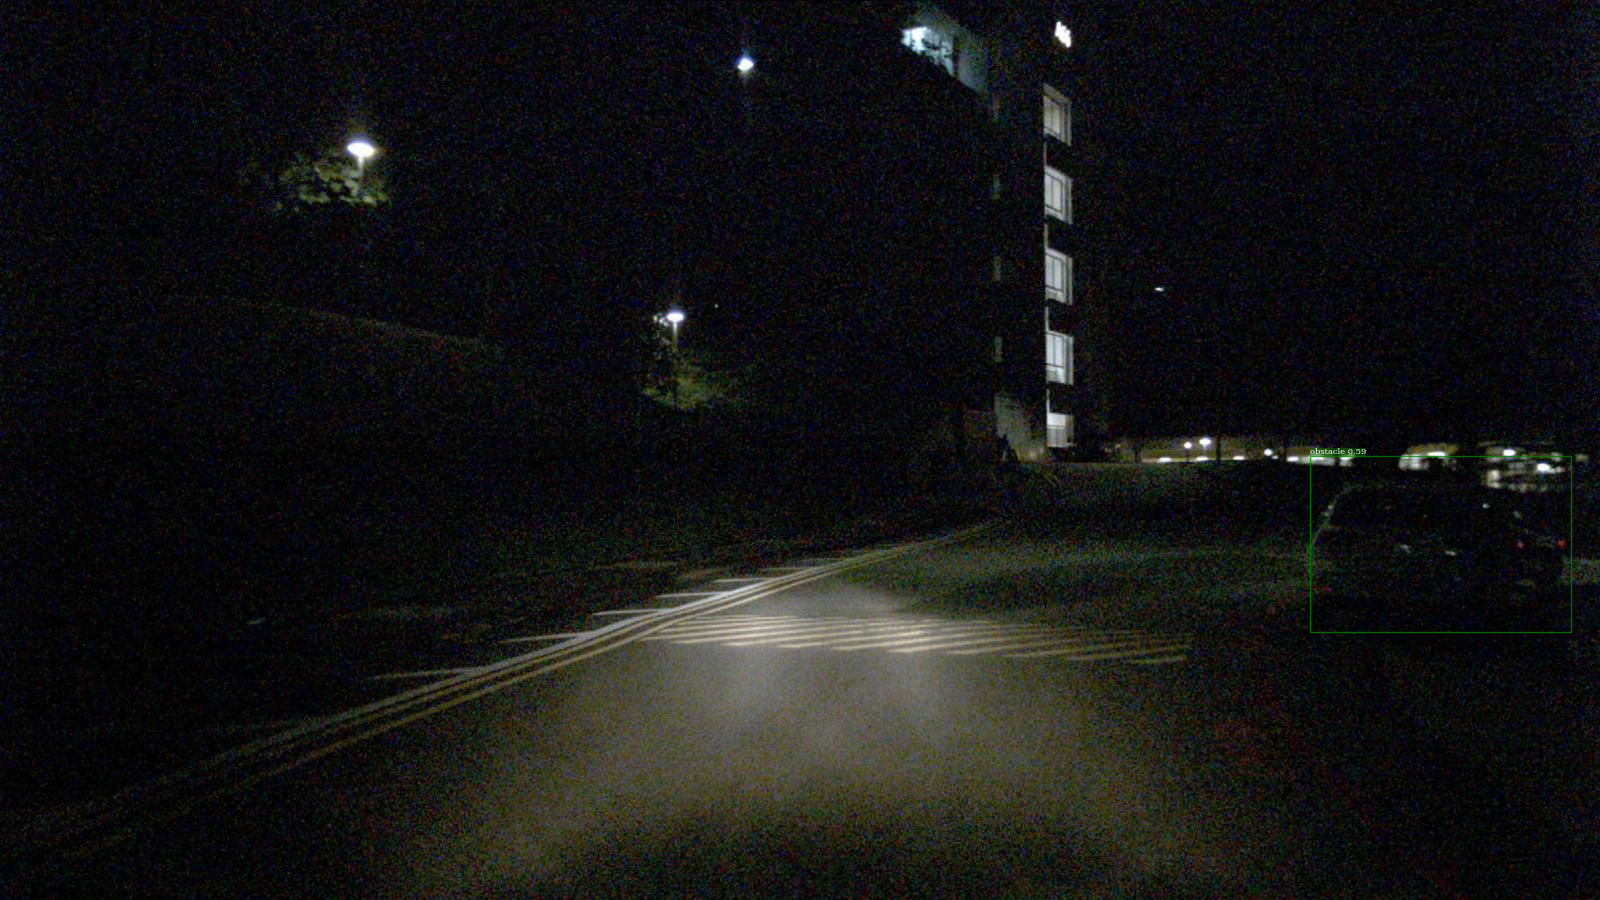
\includegraphics[width=0.3\textwidth]{images/results/saf_vs_hrfuser/samples/s4_night_reg/n015-2018-11-14-19-52-02+0800__CAM_FRONT__1542196675862460.png}
      
        % % Row 3
        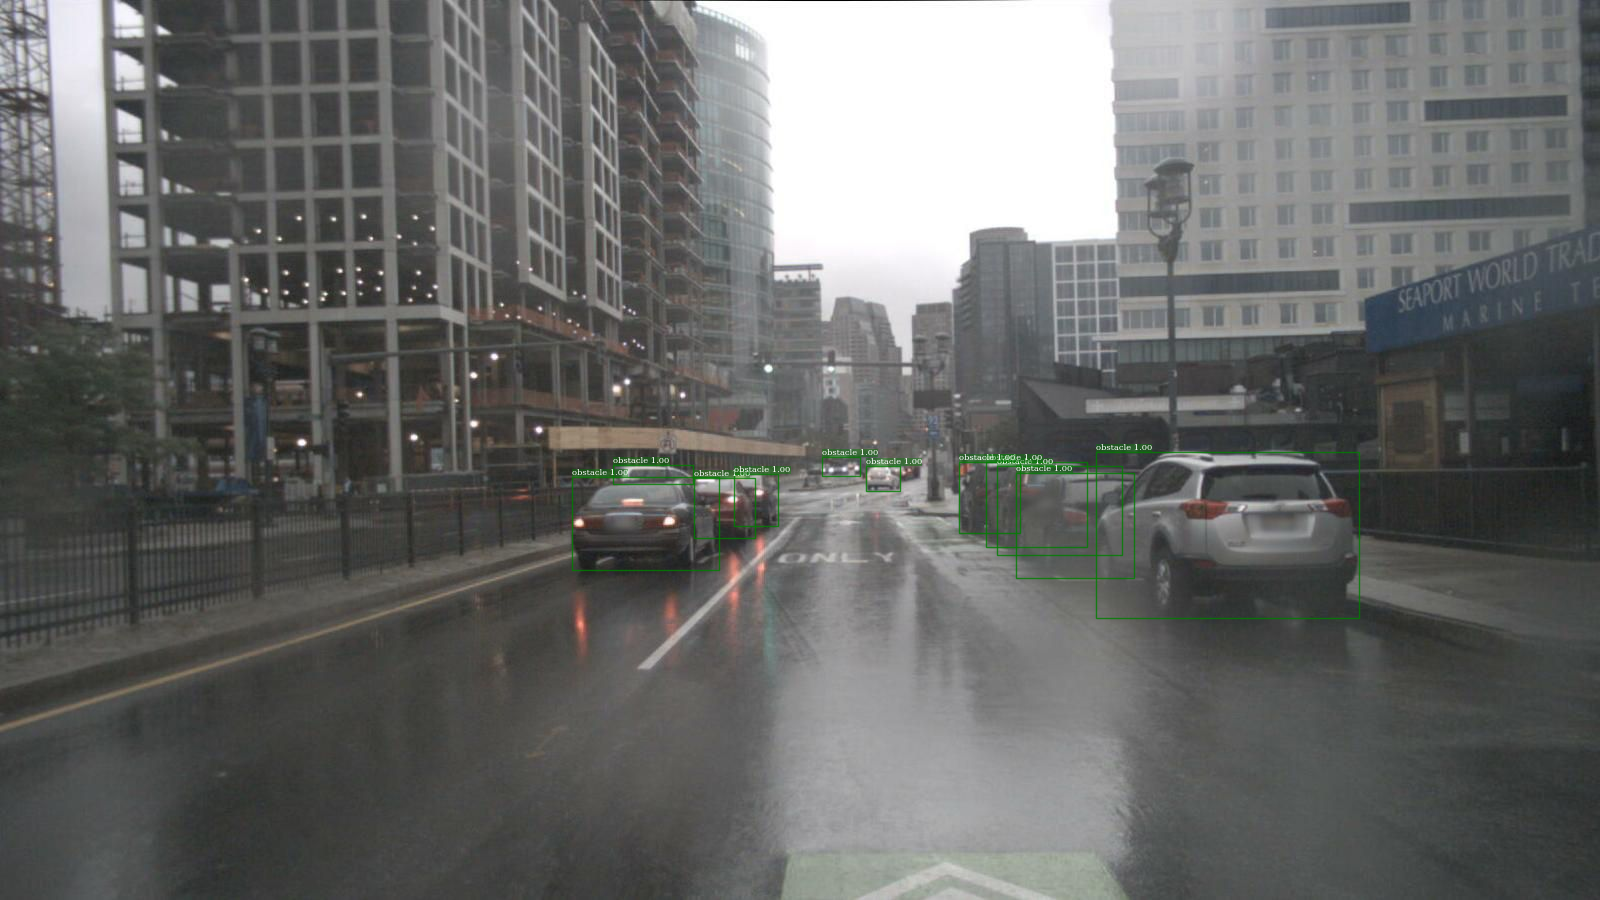
\includegraphics[width=0.3\textwidth]{images/results/saf_vs_hrfuser/samples/s5_rain_reg/n008-2018-09-18-14-18-33-0400__CAM_FRONT__1537295031112404_gt.png}\hfill
        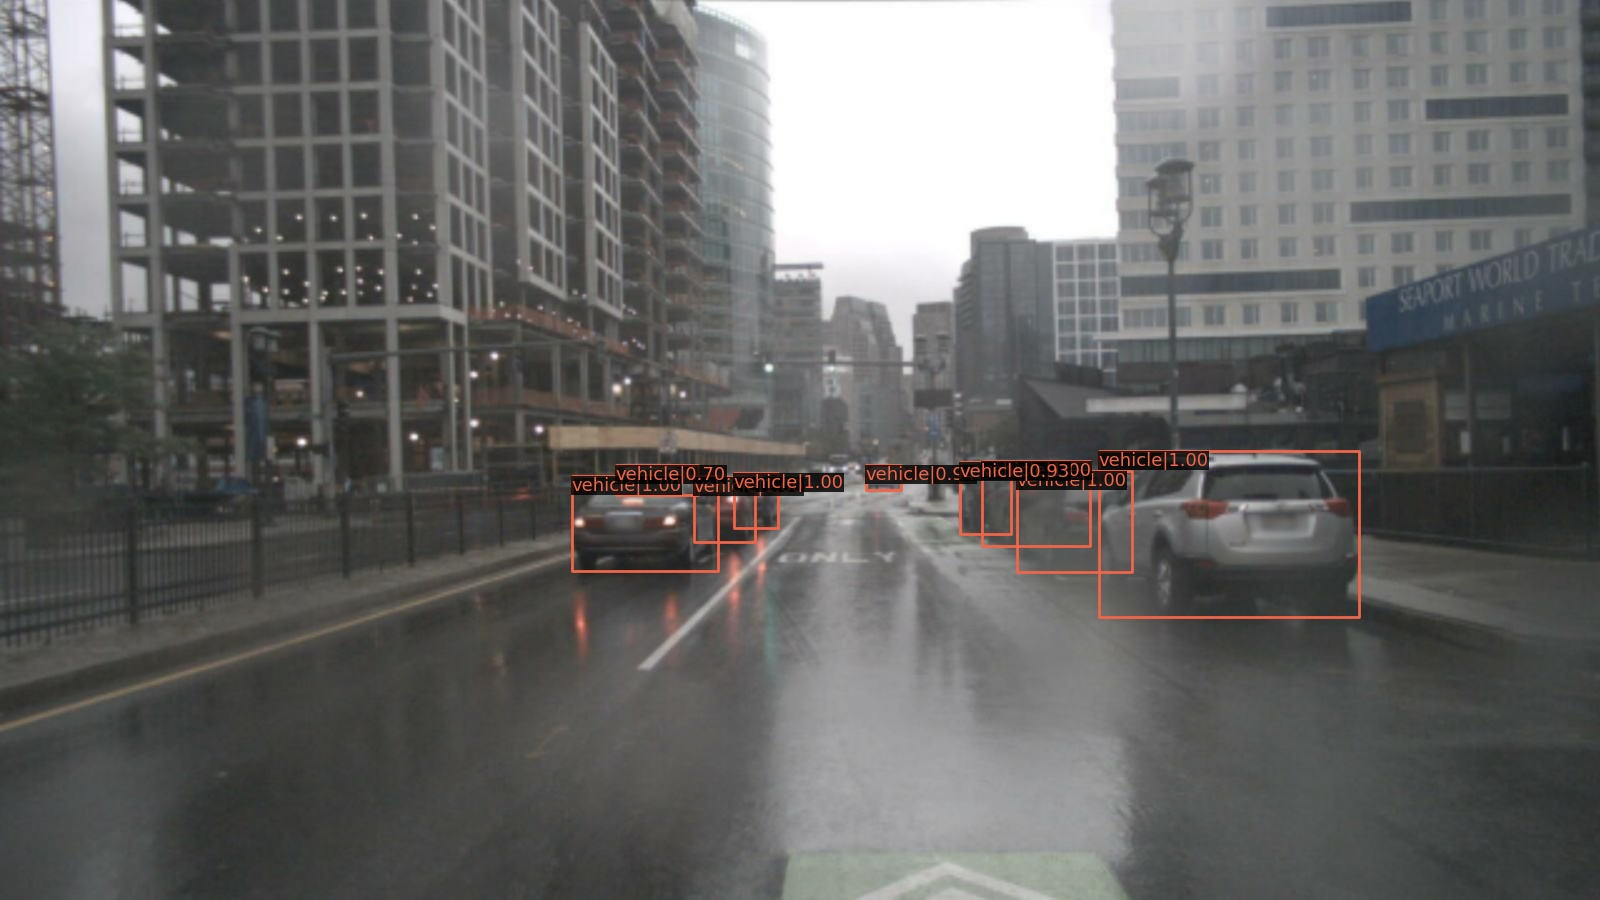
\includegraphics[width=0.3\textwidth]{images/results/saf_vs_hrfuser/samples/s5_rain_reg/n008-2018-09-18-14-18-33-0400__CAM_FRONT__1537295031112404_former.jpg}\hfill
        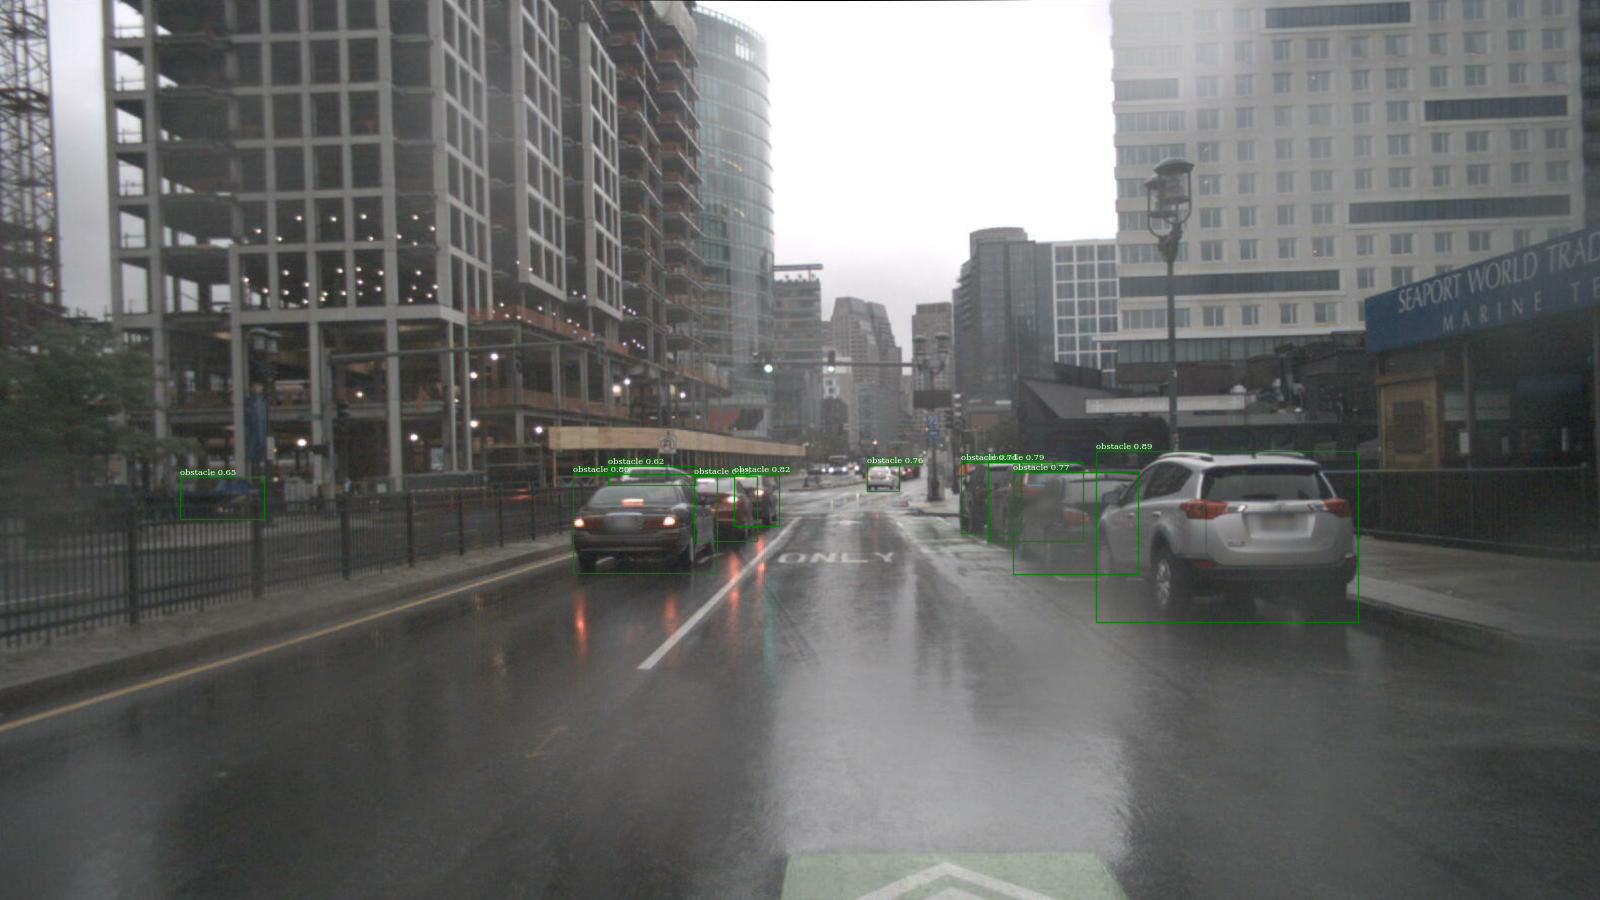
\includegraphics[width=0.3\textwidth]{images/results/saf_vs_hrfuser/samples/s5_rain_reg/n008-2018-09-18-14-18-33-0400__CAM_FRONT__1537295031112404.png}
      
        % % Row 4
        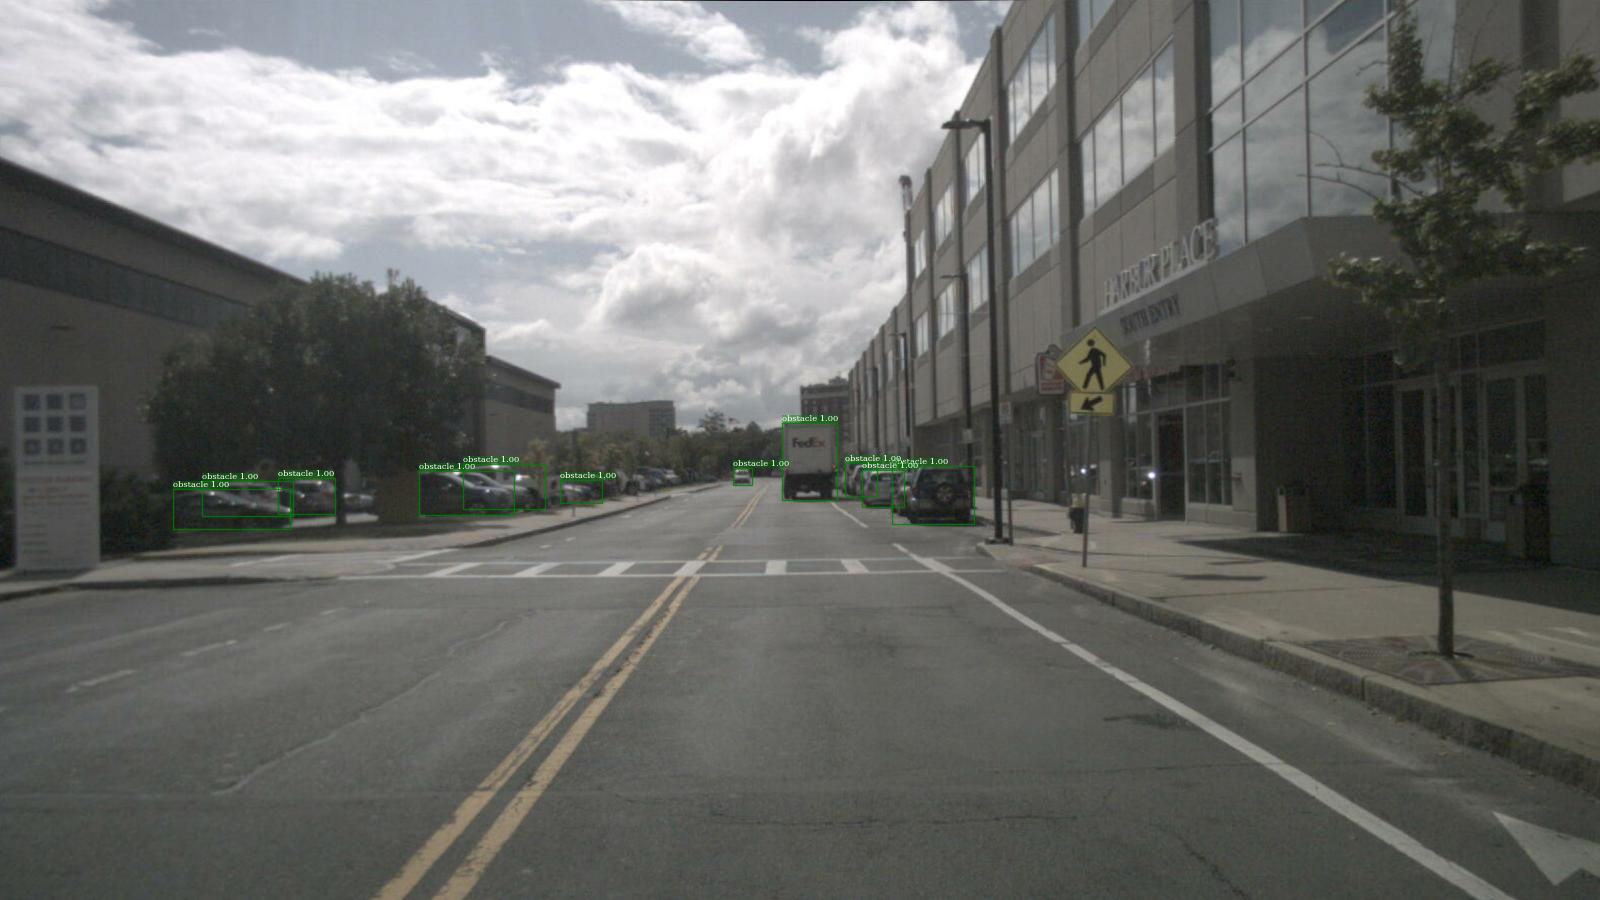
\includegraphics[width=0.3\textwidth]{images/results/saf_vs_hrfuser/samples/s1_small/n008-2018-08-01-15-34-25-0400__CAM_FRONT__1533152226912404_GT.png}\hfill
        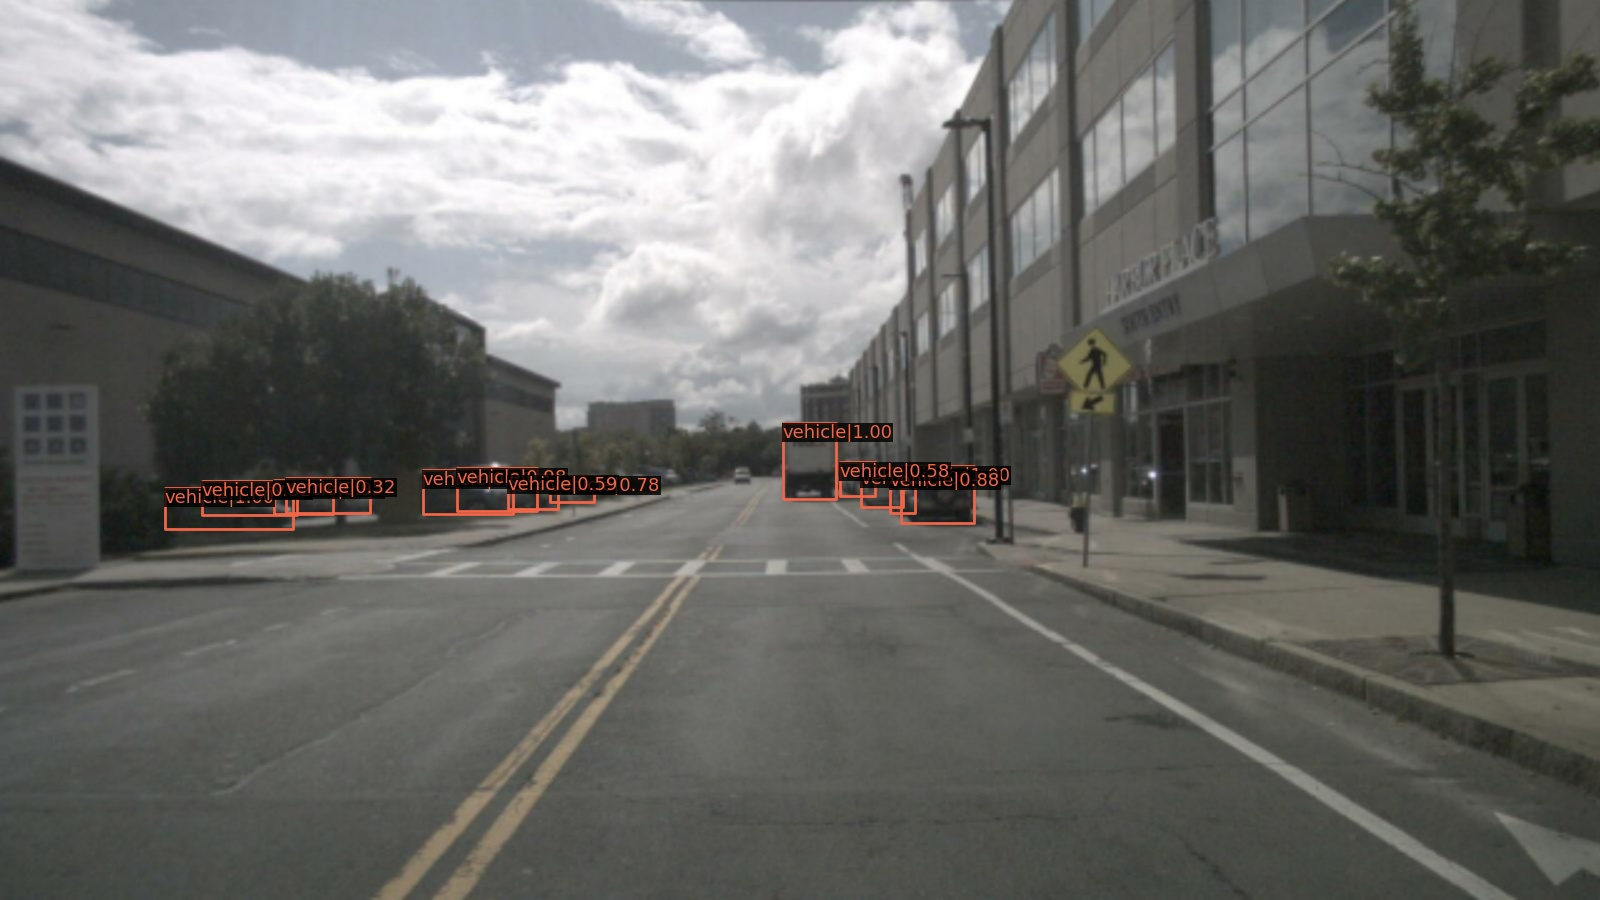
\includegraphics[width=0.3\textwidth]{images/results/saf_vs_hrfuser/samples/s1_small/n008-2018-08-01-15-34-25-0400__CAM_FRONT__1533152226912404_former.jpg}\hfill
        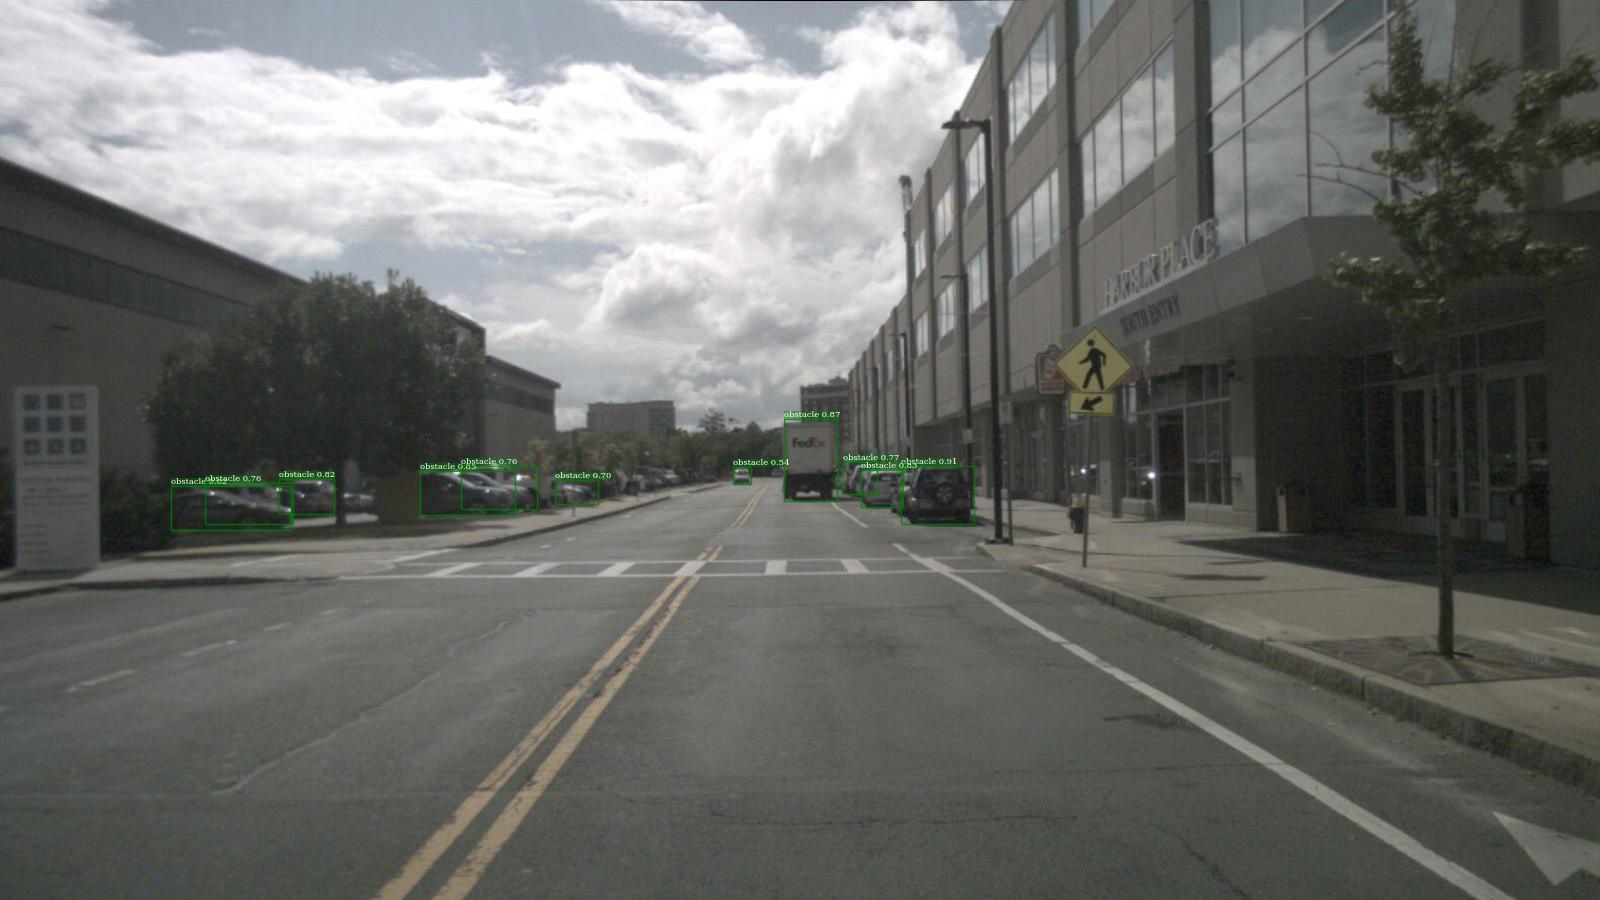
\includegraphics[width=0.3\textwidth]{images/results/saf_vs_hrfuser/samples/s1_small/n008-2018-08-01-15-34-25-0400__CAM_FRONT__1533152226912404.png}
      
        % % Row 5
        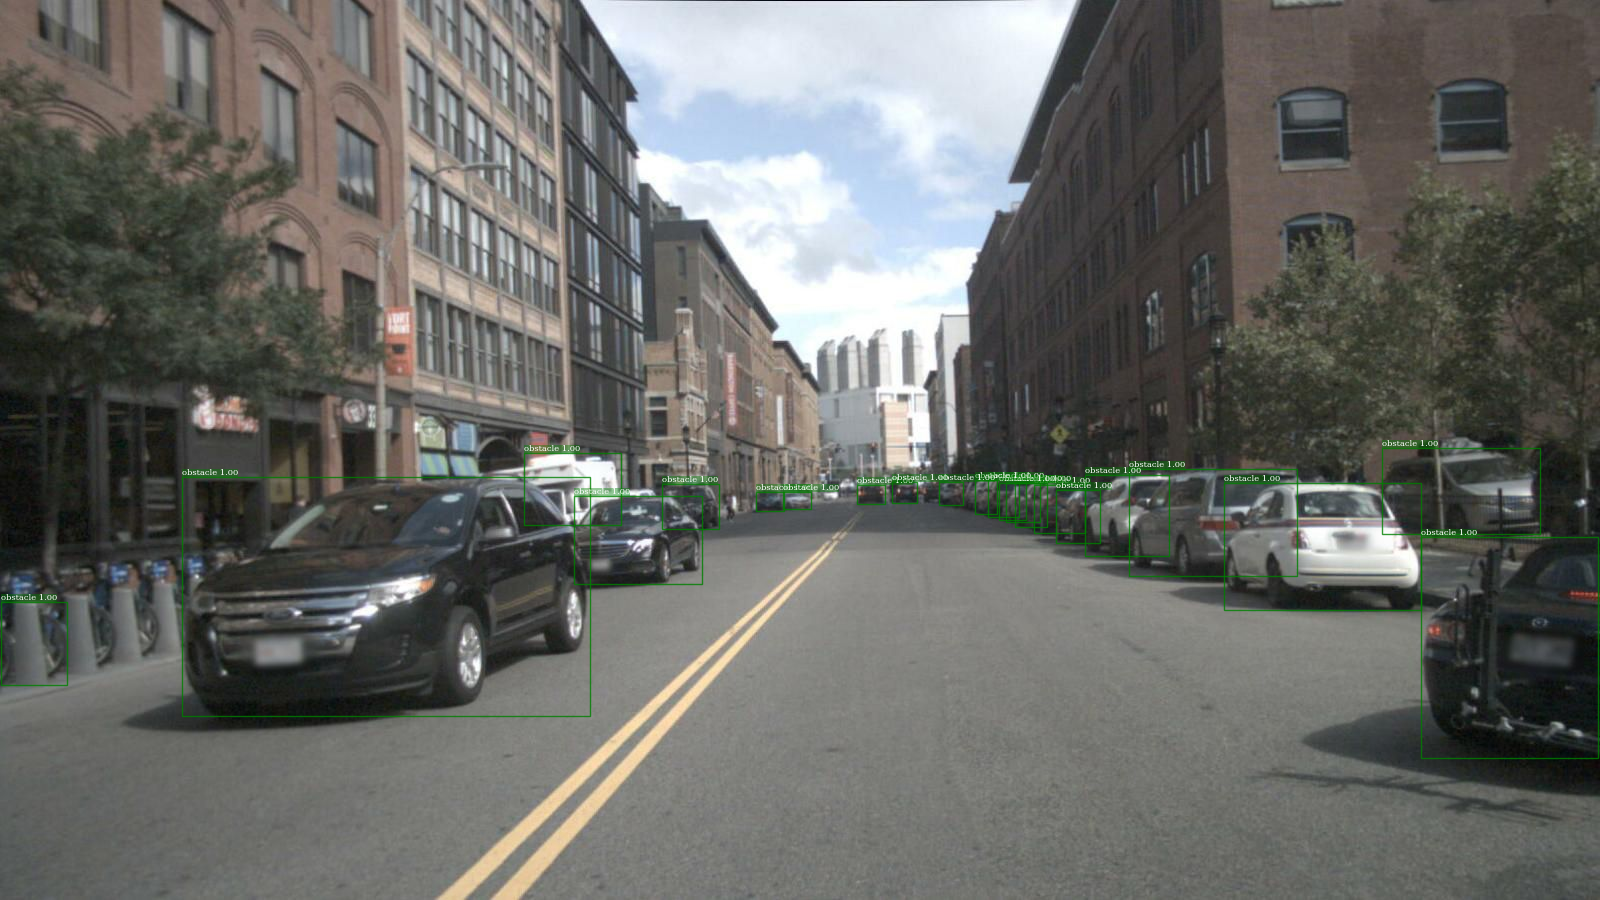
\includegraphics[width=0.3\textwidth]{images/results/saf_vs_hrfuser/samples/s2_small/n008-2018-08-01-15-34-25-0400__CAM_FRONT__1533152641412404_gt.png}\hfill
        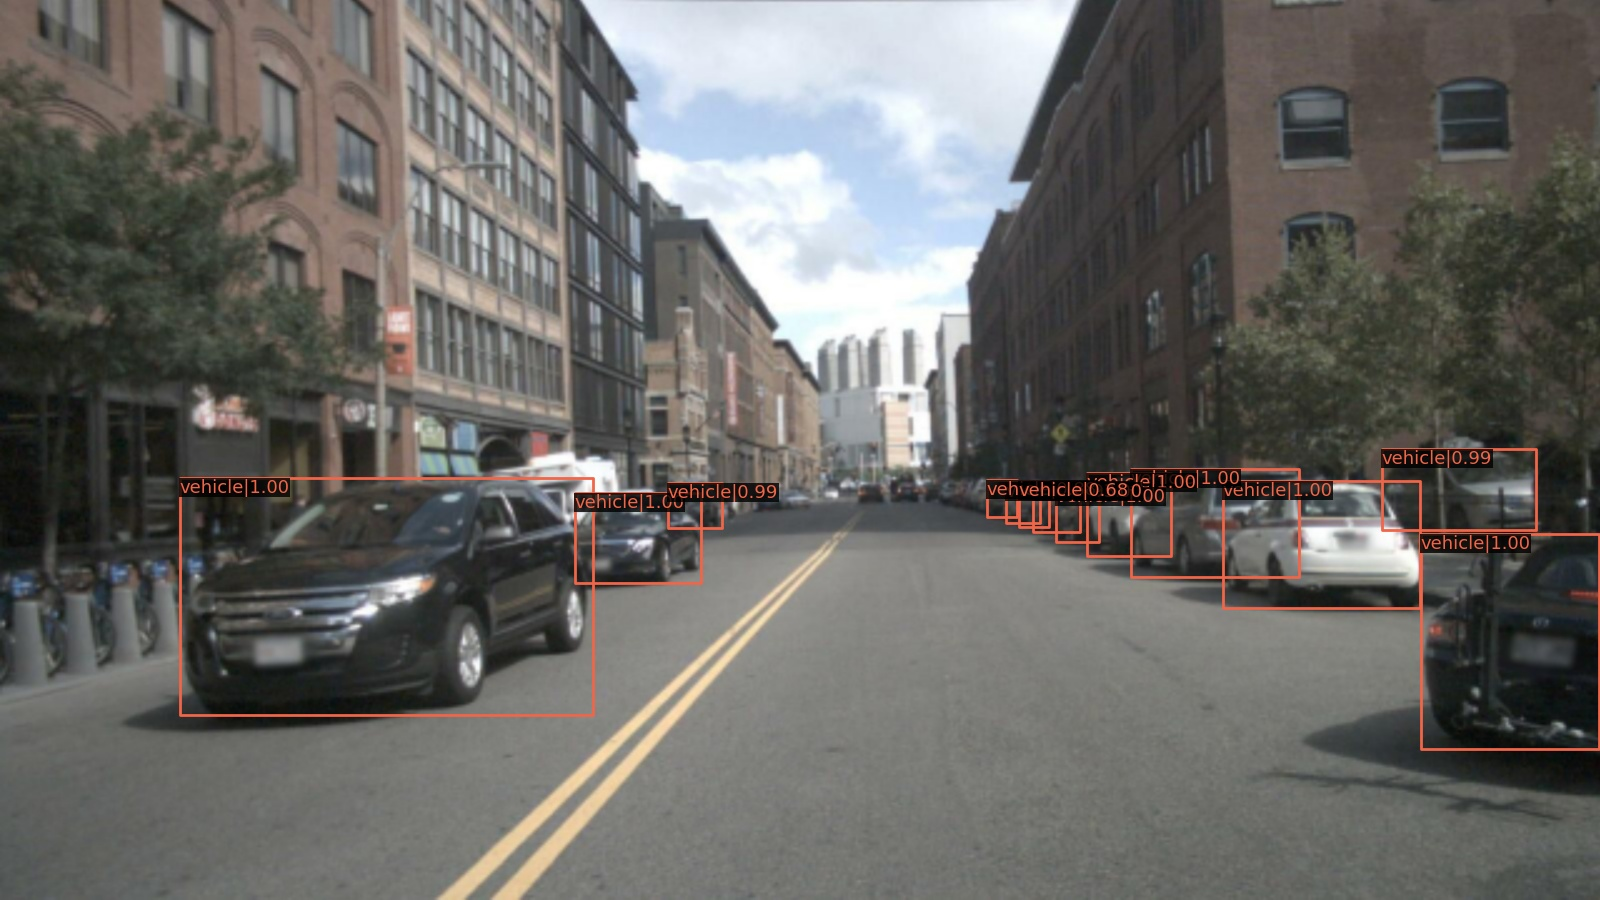
\includegraphics[width=0.3\textwidth]{images/results/saf_vs_hrfuser/samples/s2_small/n008-2018-08-01-15-34-25-0400__CAM_FRONT__1533152641412404_former.jpg}\hfill
        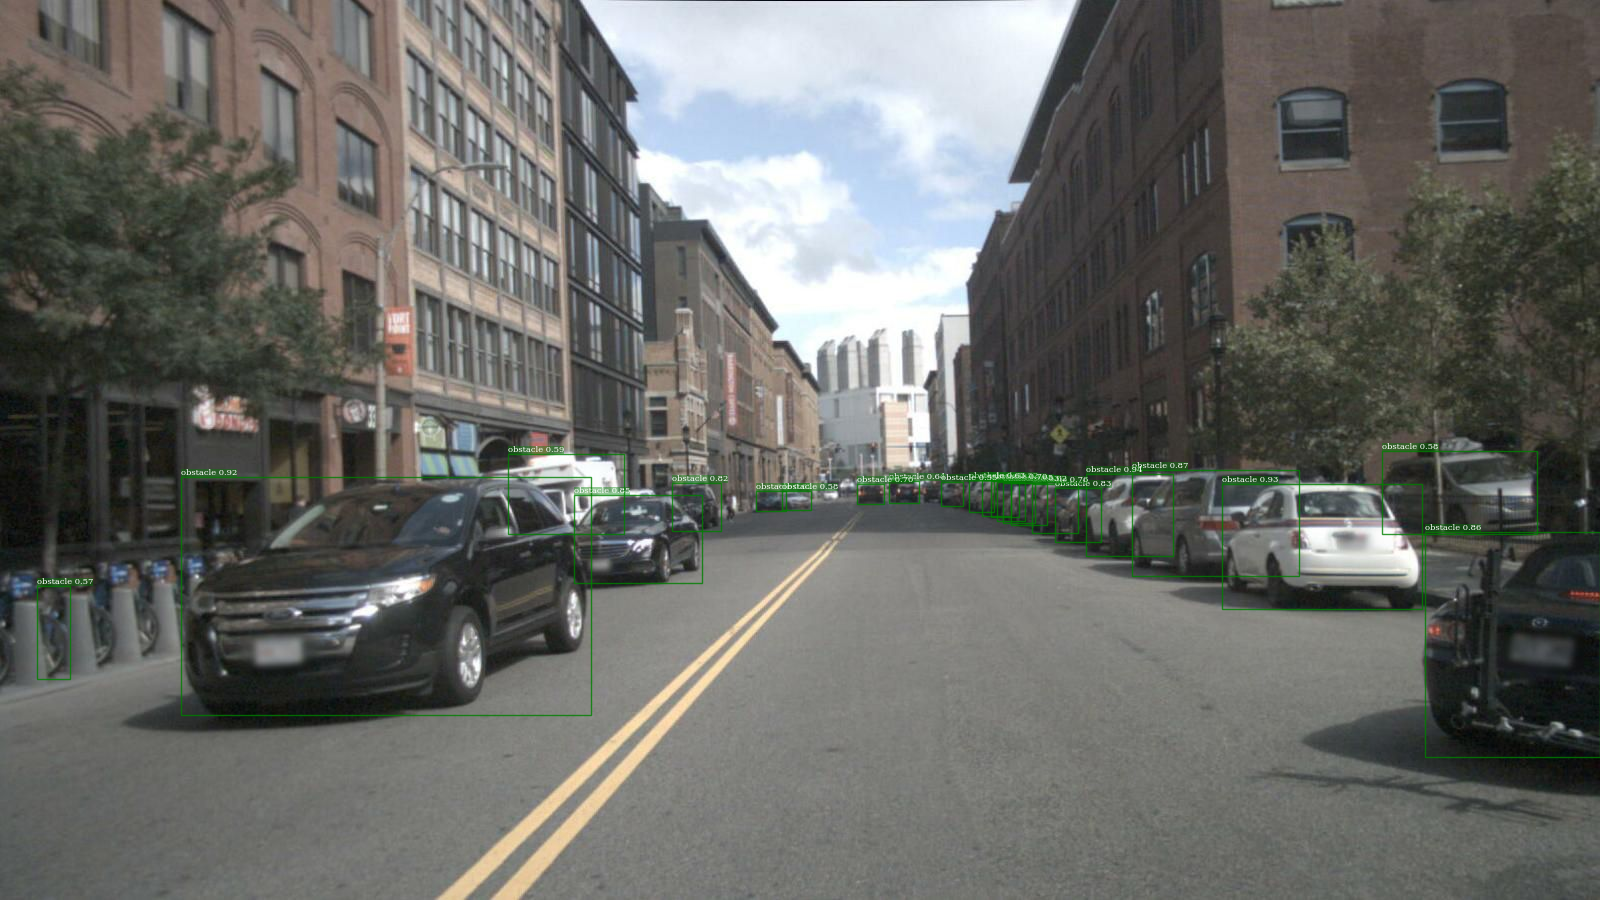
\includegraphics[width=0.3\textwidth]{images/results/saf_vs_hrfuser/samples/s2_small/n008-2018-08-01-15-34-25-0400__CAM_FRONT__1533152641412404.png}
      
        \caption{A few samples to showcase the detection results of HRFuser and SAF-FCOS. Where the 1st column is ground truth, 2nd is HRFuser, and 3rd is SAF-FCOS (1st Row: Day, 2nd Row: Night, 3rd Row: Rain, 4th and 5th Row: Small objects). Best viewed in zoomed-in view.}
        \label{fig:saf_vs_hrfuser}
      \end{figure}
    

    \subsection{Multimodal comparison with HRFuser}

    % In this section, we compare importance of different sensors when it comes to detection in adverse weather conditions on the DENSE dataset. As discussed before, the DENSE dataset covers four different sensors for environment perception namely, Camera, Radar, Lidar, and Gated infrared camera. Here, we are comparing how having complementary sensors improves the detection performance in challenging weather conditions. Both quantitative and qualitative analysis are presented in this section. Following are the comparison of only camera vs. camera+radar vs. camera+lidar vs. camera+radar+lidar and camera+radar+lidar+gated infrared camera. The results are presented in accordance with COCO-style metrics, as outlined in Table \ref{tab:coco_metrics}.

    In this analysis, we delve into the significance of varying sensor combinations for object detection under adverse weather conditions, utilizing the DENSE dataset as our benchmark. The DENSE dataset, as previously mentioned, encompasses four distinct types of sensors for environmental perception: Camera, Radar, Lidar, and a Gated Infrared Camera. This comparison focuses on assessing the enhancement in detection performance brought about by the integration of these complementary sensors. We conduct both quantitative and qualitative evaluations, comparing scenarios using only a camera, camera combined with radar, camera with lidar, a trio of camera, radar, and lidar, and finally, an amalgamation of all four sensors including the gated infrared camera. The results of these comparisons are meticulously analyzed using COCO-style metrics. This approach provides a comprehensive understanding of how each sensor contributes to the robustness of object detection in challenging weather conditions, underscoring the value of sensor fusion in enhancing environmental perception.
    



\end{document}
